\section{Modern cryptography}

\subsection{Composition of ciphers}
So far, we have seen simple historical ciphers and we have discussed how to break them. \textbf{Modern ciphers}, however, are based on very \textbf{simple operations}, such as substitution, XOR, …, that are \textbf{combined} in a smart way so to make the overall algorithm strong and really hard to analyse. It is important to keep in mind that \textbf{combining simple ciphers} does not \textbf{always} \textbf{improve security}. 

For example, consider the shift cipher composed twice. We first shift by $k_1$ and then by $k_2$ modulo 26, as represented in Picture \ref{comp1}.

\begin{figure}[h!]
        \centering
        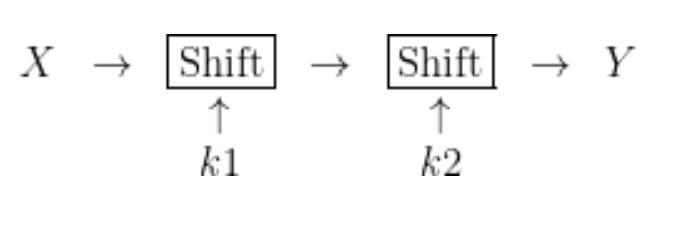
\includegraphics[scale = 1.0]{img/comp1.png}
        \label{comp1}
        \caption{Composition of two shift ciphers - 1}
\end{figure}

It is clear that this is equivalent to shifting by $k_1+k_2$ modulo 26, meaning that applying twice the cipher is the same as applying it once with a key given by the sum of the two keys.

\begin{figure}[h!]
        \centering
        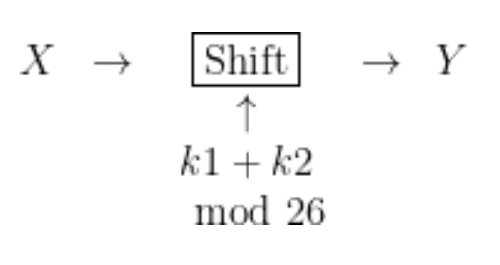
\includegraphics[scale = 1.0]{img/comp2.png}
        \label{comp2}
        \caption{Composition of two shift ciphers - 2}
\end{figure}

This informal reasoning can be made more precise.

\textbf{Definition (Composition)}. We consider two ciphers $S^1=({\cal P}^1,{\cal C}^1,{\cal K}^1,E^1,D^1)$ and $S^2=({\cal P}^2,{\cal C}^2,{\cal K}^2,E^2,D^2)$. We let ${\cal P}^1={\cal C}^1={\cal P}^2={\cal C}^2$, that we note as ${\cal P}$ and ${\cal C}$ in the following. In this way the output of one cipher is for sure a possible plaintext for the second cipher. We can now define \textbf{composition} as $S^1 \times S^2 = ({\cal P},{\cal C},{\cal K}^1\times{\cal K}^2,E,D)$ with

$$
E_{(k1,k2)}(x) = E^2_{k2}(E^1_{k1}(x))
$$

$$
D_{(k1,k2)}(y) = D^1_{k1}(D^2_{k2}(y))
$$

As we can see, in order to encrypt a plaintext $x$ using a composition of two ciphers with keys $k1$ and $k2$ we must:

\begin{enumerate}
    \item \textbf{Encrypt} $x$ using the \textbf{first encryption function} (using $k1$);
    \item \textbf{Encrypt} the \textbf{result} of (1) using the \textbf{second encryption function} (using $k2$).
\end{enumerate}

\example{Consider the composition of the two shifts above. Formally we have that $E^1_k(x) = E^2_k(x) = x+k \mod 26$. Thus,\begin{equation}\begin{align*}E_{(k1,k2)}(x) &= E^2_{k2}(E^1_{k1}(x)) = (x + k1 \mod 26) + k2 \mod 26\\ &= x + (k1+k2 \mod 26) \mod 26 = E^1_{k1+k2 \mod 26}(x)\end{align*}\end{equation}This proves that composing the shift cipher twice is equivalent to applying it once using as a key the sum of the two keys $k1$ and $k2$, modulo 26.}

\subsubsection{Idempotent ciphers}
We have seen that the shift cipher, when repeated twice is equivalent to itself with a different key. When this happens, the cipher $S$ is said to be \textbf{idempotent}, written $S \times S = S$. In this case we know that iterating the cipher will be of no use to improve its security. Even if we repeat it $n$ times we will still get the initial cipher, i.e., $S^n = S$.

We have mentioned that modern ciphers are based on simple operations composed together. Another ingredient is, in fact, \textbf{iteration}. Almost any modern cipher repeats a \textbf{basic core of operations} for a certain number of \textbf{rounds}. It is thus necessary that such core operations do not constitute an idempotent cipher.

It can be proved that if we have two \textbf{idempotent} \textbf{ciphers} that commute, i.e., such that $S^1 \times S^2 = S^2 \times S^1$, then their \textbf{composition} is also \textbf{idempotent}. In this case, we know that iterating their composition is useless. To see why this holds consider one iteration of their composition (recall that function composition is associative):

$$
\begin{array}{ll}(S^1 \times S^2) \times (S^1 \times S^2)\\ = S^1 \times (S^2 \times S^1) \times S^2 &\mbox{ associative property}\\ = S^1 \times (S^1 \times S^2) \times S^2 &\mbox{ commutative property}\\= (S^1 \times S^1) \times (S^2 \times S^2) &\mbox{ associative property}\\ = S^1 \times S^2 &\mbox{ idempotence of the initial ciphers} \end{array}
$$

\subsubsection{Recap}
We have seen examples of how algebraic properties, such as commutativity, can help simplifying the analysis of a cipher. When developing a robust cipher we need to avoid as much as possible that operations can be rearranged, swapped, simplified.

\subsection{The AES cipher}
The \textbf{Advanced Encryption Standard} (AES) has been selected by the National Institute of Standards and Technology (NIST) after a five-year long competition. The original name of the cipher is Rijndael from the names of the two inventors, the cryptographers Joan Daemen and Vincent Rijmen. As any modern cipher, AES is the \textbf{composition} of rather \textbf{simple operations} and contains a \textbf{non-linear component} to \textbf{avoid} \textbf{known-plaintexts attacks} (as the one we have seen on the Hill cipher). The composed operations give a \textbf{non-idempotent cipher} that is \textbf{iterated} for a fixed number of \textbf{rounds} (the longer the key, the more rounds are executed).

Rijndael has been selected because it resulted to be the best one providing:

\begin{itemize}
    \item High \textbf{security} guarantees;
    \item High \textbf{performance};
    \item \textbf{Flexibility} (different key length).
\end{itemize}

All of these \textbf{features} are, in fact, \textbf{crucial} for any modern cipher. Its predecessor, the Data Encryption Standard (DES) is still in use after almost 40 years, in a variant called Triple DES (3DES), which aims at improving the key length. In fact, DES key of only 56 bits is too short to resist brute-forcing on modern, parallel computers.

\subsubsection{Mathematical background}
AES works on the \textbf{Galois Field} with $2^8$ elements noted $\mathbf{GF}(2^8)$. Intuitively, it is the \textbf{set} of all \textbf{8-bit digits} with \textbf{sum} and \textbf{multiplications} performed by interpreting the bits as (binary) \textbf{coefficients of polinomials}. For example, element $11010011$ can be seens as $x^7 + x^6 + x^4 + x + 1$ while $00111010$ is $x^5+x^4+x^3 + x$. The sum will thus be $x^7+x^6+x^4+x+1+x^5+x^4+x^3+x=x^7+x^6+x^5+x^3+1$, since two 1’s coefficient becomes 0, modulo 2, and the term disappears (for example $x + x = 2x = 0x = 0$). We see that \textbf{sum} and \textbf{subtraction} are just the \textbf{bit-wise XOR} of the binary numbers, i.e., $11010011 \oplus 00111010 = 11101001$ which is $x^7+x^6+x^5+x^3+1$.

\textbf{Product} is done \textbf{modulo} the \textbf{irreducible polinomial} $x^8 + x^4 + x^3 + x + 1$. Irreducible means that it cannot be written as the product of two other polinomials (it is, intuitively, the equivalent of primality). 

For example, $(x^7 + x^6 + x^4 + x + 1) \times (x^5+x^4+x^3 + x)$ gives

$$x^{12} + x^{11} + x^9 + x^6 + x^5+x^{11}+x^{10}+x^8+x^5+x^4+x^{10}+x^9+x^7+x^4+x^3+x^8+x^7+x^5+x^2+x$$

, which is reduced to

$$x^{12}+x^6+x^5+x^3+x^2+x$$

Now, the next step is to \textbf{divide} $x^{12}+x^6+x^5+x^3+x^2+x$ by the \textbf{irreducible polynomial} $x^8 + x^4 + x^3 + x + 1$, and find the remainder. In general, long division of polynomials is similar to long division of whole numbers, and when we divide two polynomials we can check the answer using:

$$
\text{dividend} = (\text{quotient} \cdot \text{divisor}) + \text{remainder}
$$

or, equivalently,

$$
\text{dividend} / \text{divisor} = \text{quotient} + \frac{\text{remainder}}{\text{divisor}} 
$$

In our example, dividing $x^{12}+x^6+x^5+x^3+x^2+x$ by $x^8 + x^4 + x^3 + x + 1$ and finding the remainder results as follows:

\begin{enumerate}
    \item Since $x^{12}/x^8 = x^4$, we shift 4 bits to the left the divisor;
    \item Then, we perform a XOR operation between the dividend and the divisor;
    \item Since the results contains 9 bits, which is too much, we perform another XOR operation between the previous result and the divisor;
    \item Finally, we retrieve the remainder, which results to be $11000101$, i.e., $x^7 + x^6 + x^2 + 1$.
\end{enumerate}

$$
\begin{array}{ccccccccccccc}1&0&0&0&0&0&1&1&0&1&1&1&0 \\ 1&0&0&0&1&1&0&1&1 \\\hline & & & &1&1&1&0&1&1&1&1&0\\ & & & &1&0&0&0&1&1&0&1&1 \\\hline & & & & &1&1&0&0&0&1&0&1 \end{array}
$$

This operation is \textbf{quadratic} in general, with respect to the number of bits (8). It can be optimized with the following linear algorithm (which is, in fact, a working python code):

\begin{figure}[h!]
        \centering
        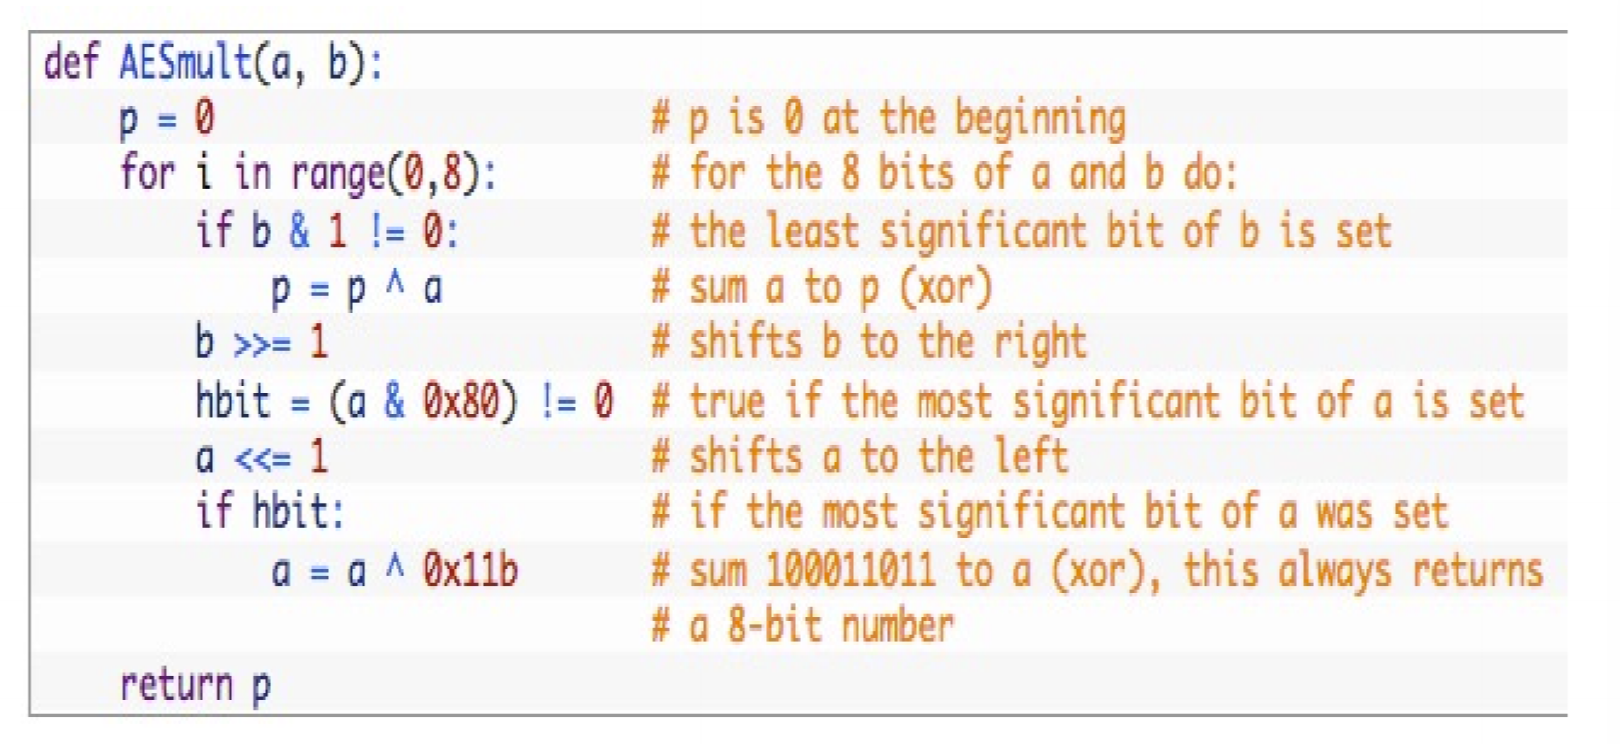
\includegraphics[scale = 0.8]{img/aes1.png}
        \label{aes1}
        \caption{Product - optimization}
\end{figure}

The \textbf{optimization} works as follows:

\begin{enumerate}
    \item We let $a$ to be the binary representation of the coefficients of the first term of the multiplication, and $b$ the binary representation of the coefficients of the second one;
    \item We let $p = 00$;
    \item We perform a XOR operation between $a$ and $p$, and we update $p$ with the result of this operation;
    \item Then, $b$ is shifted to the right and $a$ is shifted to the left meaning that we respectively divide and multiply by $x$ the two polynomials. Now we erase the least significant bit of $b$ and we add a 0 to $a$:
    \begin{itemize}
        \item If the least significant bit is a 1, we continue performing the XOR operation between the new $a$ and $p$;
        \item Otherwise, we skip the XOR operation. 
    \end{itemize}
    \item When $a$ becomes more than $2^8$ we need to XOR to it the modulus $100011011$, i.e. $0x11b$, to keep it 8-bits long.
\end{enumerate}

An example is provided in Picture \ref{aes8}.

\begin{figure}[h!]
        \centering
        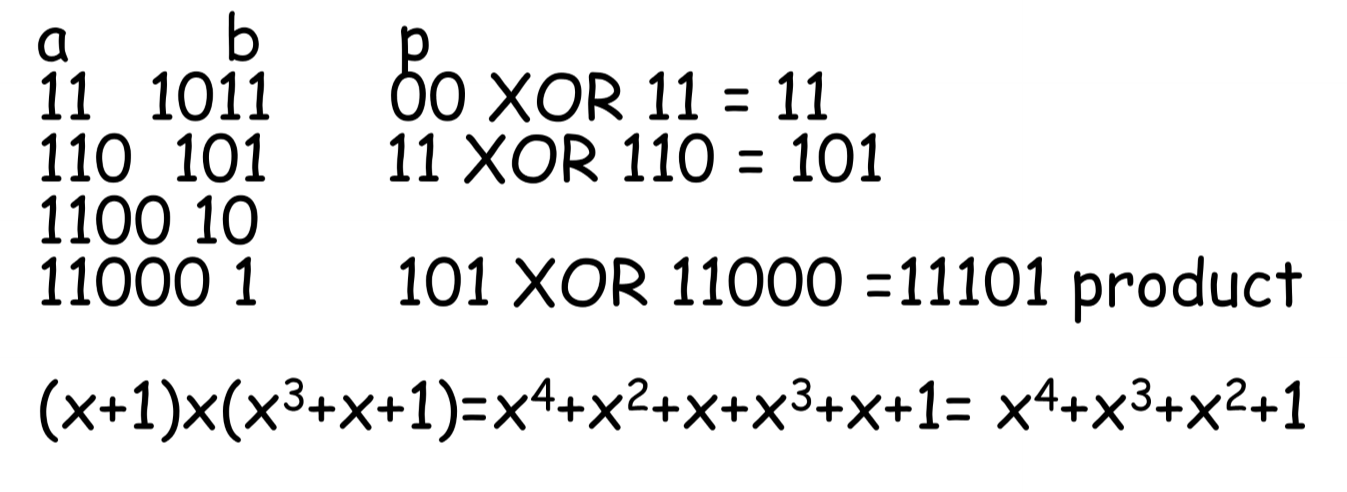
\includegraphics[scale = 0.65]{img/aes8.png}
        \label{aes8}
        \caption{Product - optimization: example}
\end{figure}

The \textbf{correctness} of this algorithm derives from the \textbf{invariant} which states that after each loop: 

\begin{itemize}
    \item $ab+p$ is the product of the initial $a$ and $b$ (all operation does in the Galois Field);
    \item Since $b$ is 0 at the end, we have that $p$ will contain the product.
\end{itemize}

\subsubsection{The AES cipher}
Now that we have introduced the basic operation used to implement AES we can describe the cipher. The official \textbf{description} of \textbf{AES} is available on-line.

AES operates on a \textbf{4×4 matrix} of bytes. We have that 16 bytes are 128 bits which is, in fact, the block size. \textbf{Plaintext} bytes $b_1,\ldots,b_{16}$ are copied in the matrix by columns following this scheme:

$$  \begin{bmatrix}b_1&b_5&b_9&b_{13}\\b_2&b_6&b_{10}&b_{14}\\b_{3}&b_7&b_{11}&b_{15}\\b_4&b_8&b_{12}&b_{16}
    \end{bmatrix}
$$

Cipher \textbf{keys} have lengths of 128, 192, and 256 bits. AES has \textbf{10 rounds} for 128-bit keys, \textbf{12 rounds} for 192-bit keys, and \textbf{14 rounds} for 256-bit keys. Rijndael was designed to handle additional block sizes and key lengths, however they are not adopted in the AES standard. A round is composed of different operations, all of which are invertible:

\begin{enumerate}
    \item \textbf{AddRoundKey}: the round \textbf{key} (see Key Expansion, below) is bitwise \textbf{XOR}-ed with the \textbf{block}. A round key is thus 128 bits, independently of the chosen key size.

    \begin{figure}[h!]
        \centering
        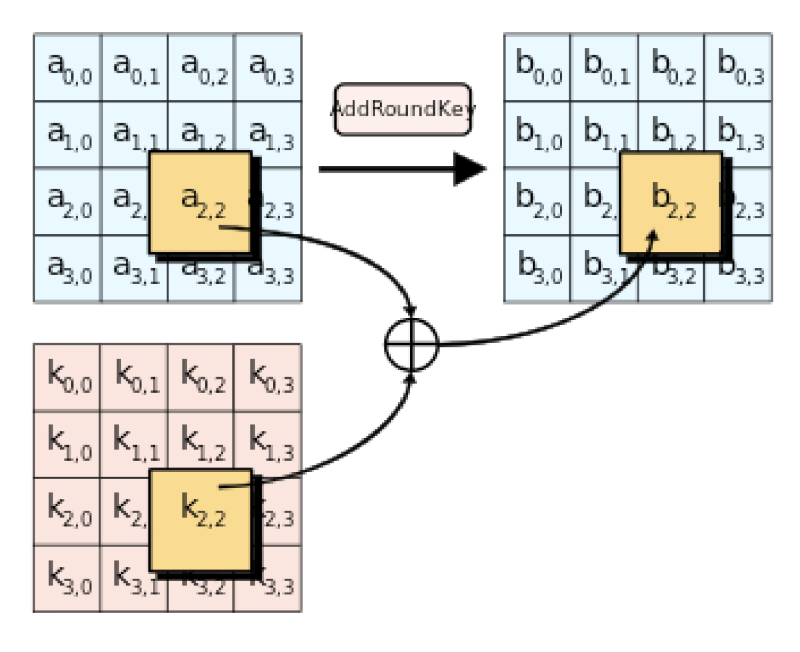
\includegraphics[scale = 0.8]{img/aes2.png}
        \label{aes2}
        \caption{AddRoundKey operation}
    \end{figure}

    In this example, $b_{2,2} = a_{2,2} \text{ XOR } k_{2,2}$.
    
    \item \textbf{SubBytes}: a \textbf{fixed }\textbf{non-linear substitution}, called \textbf{S-box}, is applied to each byte of the block. The substitution is reported below. Given a \textbf{byte} in hexadecimal notation, the \textbf{first digit} is used to select a \textbf{row} and the \textbf{second} one to select a \textbf{column}. For example, $0x25$ would be the third row (2) and the sixth column (5) giving $0x3f$.

    \begin{figure}[h!]
        \centering
        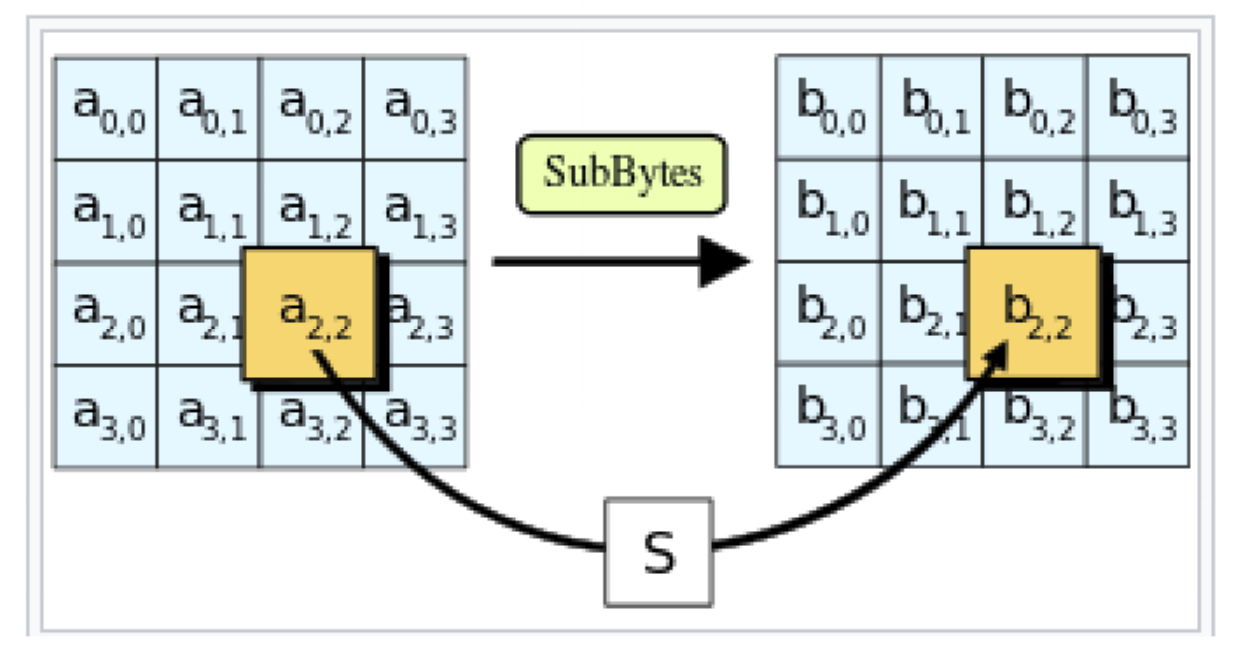
\includegraphics[scale = 0.65]{img/aes3.png}
        \label{aes2}
        \caption{SubBytes operation}
    \end{figure}

    The S-box is represented below:

    \begin{figure}[h!]
        \centering
        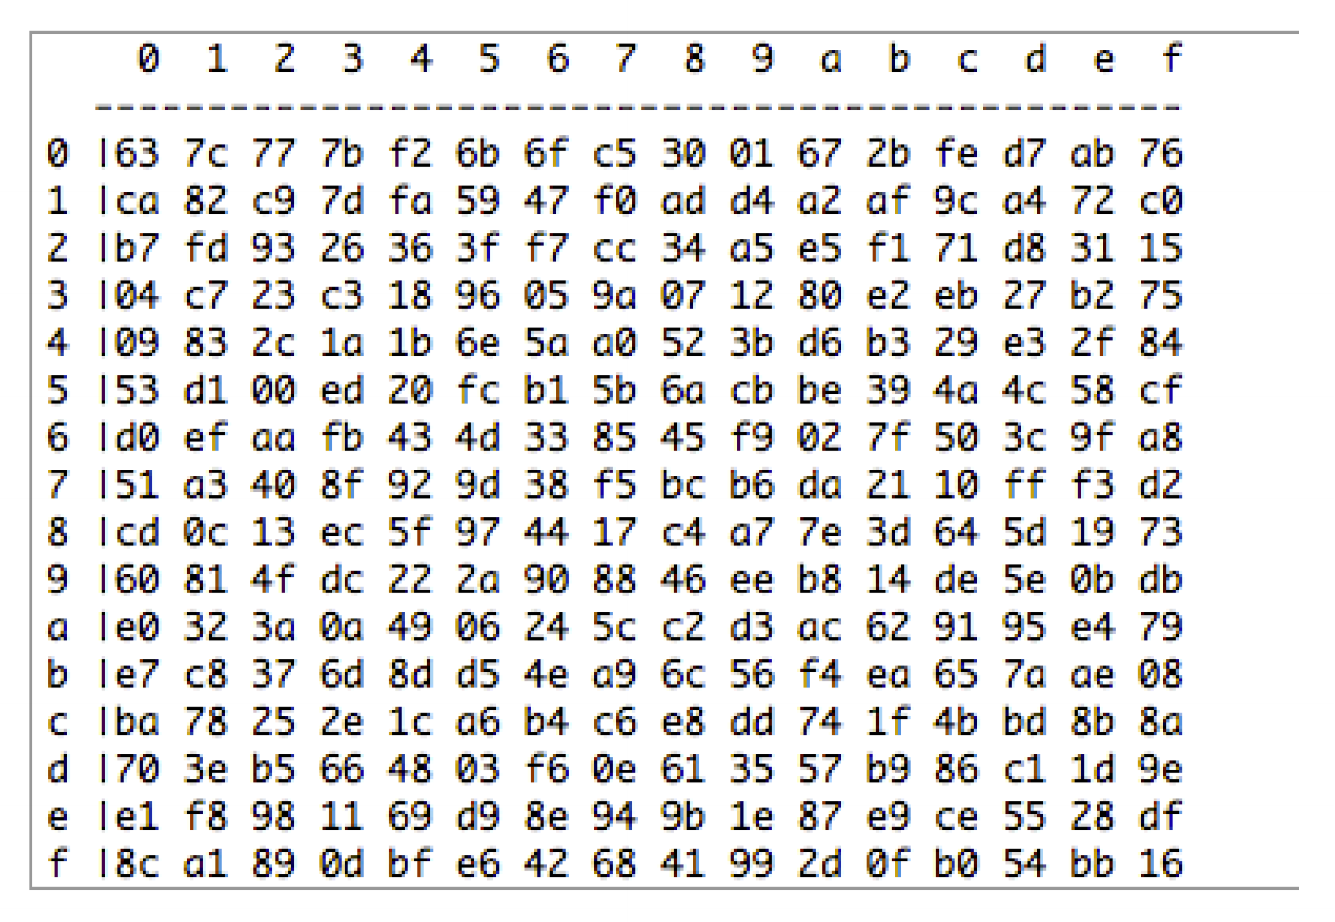
\includegraphics[scale = 0.8]{img/aes4.png}
        \label{aes4}
        \caption{S-box}
    \end{figure}

    Notice that S-box is secure because the attacker cannot easily retrieve $b_{2,2}$, since $2^{16}$ possible values exist. Moreover, this S-box has been obtained by taking, for each byte, its \textbf{multiplicative inverse} in the finite field (that can be computed efficiently via an algorithm that we will see later on), noted $b_7, \ldots, b_0$, and applying the affine transformation $b_i = b_i \oplus b_{i+4 \mod 8} \oplus b_{i+5 \mod 8} \oplus b_{i+6 \mod 8}\oplus b_{i+7 \mod 8} \oplus c_i$, with $c_i$ representing the i-th bit of $01100011$. The above transformation can be written as:

    \begin{figure}[h!]
        \centering
        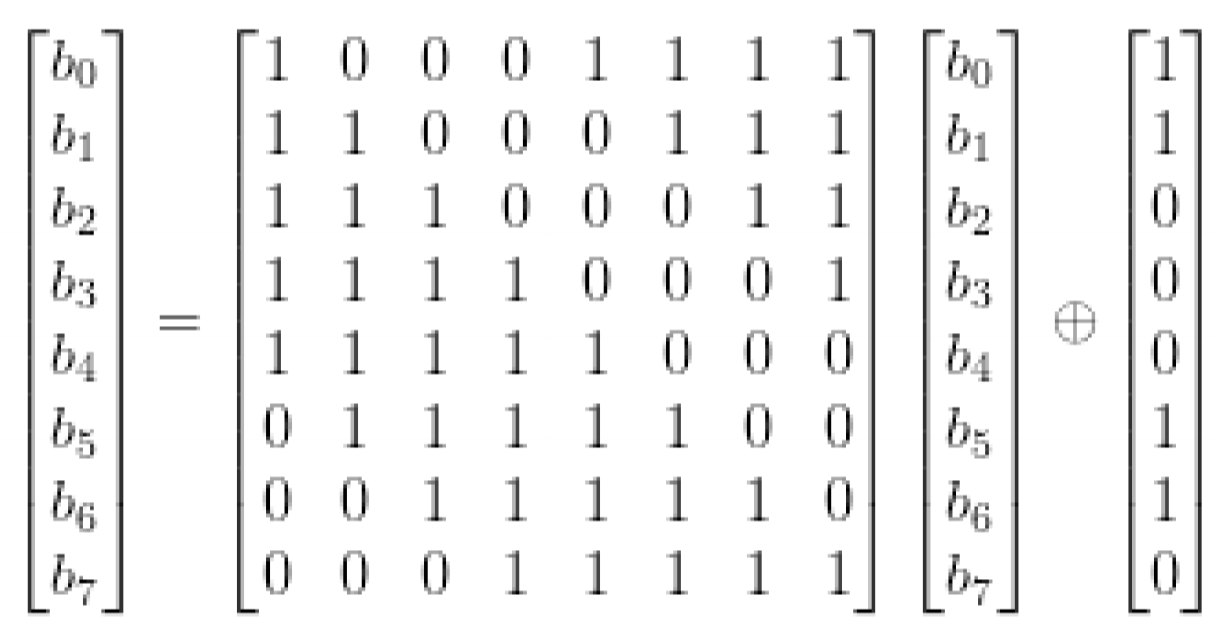
\includegraphics[scale = 0.65]{img/aes5.png}
        \label{aes5}
        \caption{Generation of the S-box}
    \end{figure}

    Using multiplicative inverses is known to give \textbf{non-linear properties}, while the affine transformation complicates the attempt of algebraic reductions.

    \item \textbf{ShiftRows}: \textbf{rows} of the block matrix are \textbf{shifted} to the left by 0,1,2,3, respectively. The shift is circular:

    \begin{figure}[h!]
        \centering
        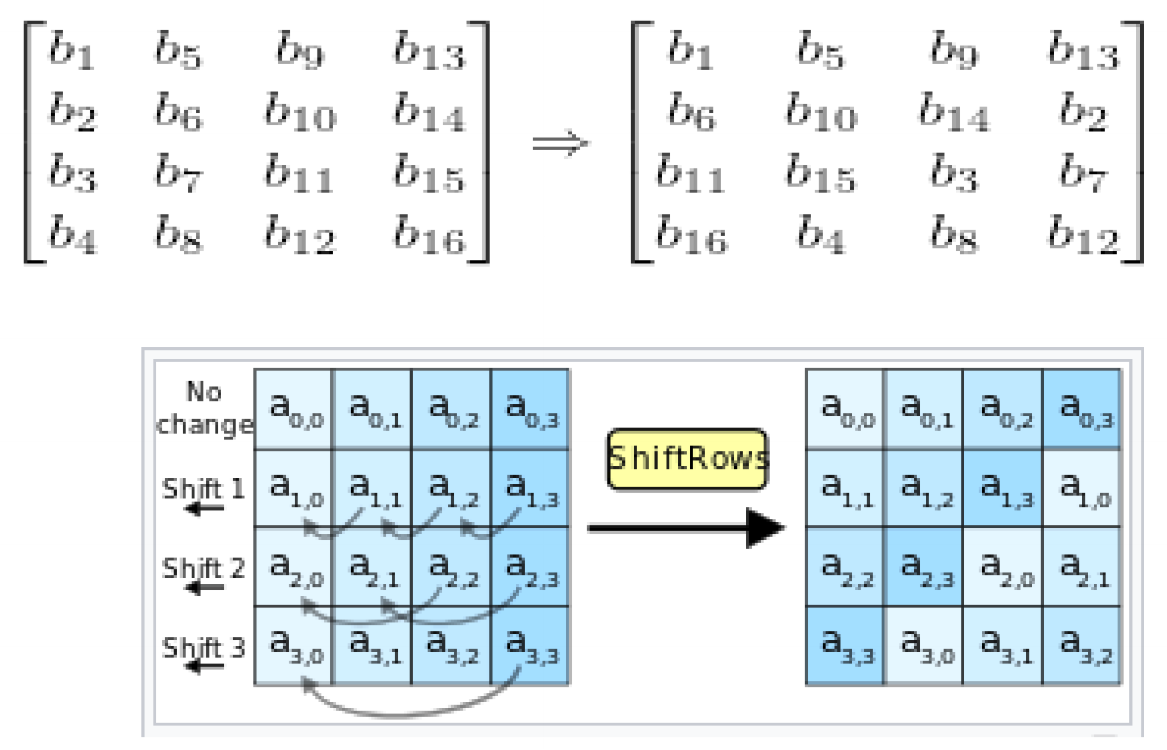
\includegraphics[scale = 0.8]{img/aes6.png}
        \label{aes6}
        \caption{ShiftRows operation}
    \end{figure}

    \item \textbf{MixColumns}: columns of the block matrix are multiplied by the following matrix:

    \begin{figure}[h!]
        \centering
        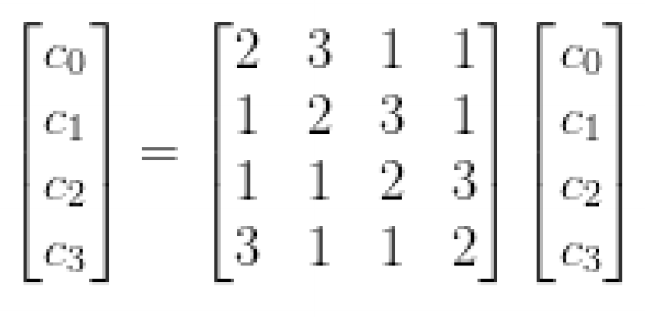
\includegraphics[scale = 0.8]{img/aes7.png}
        \label{aes7}
        \caption{MixColumns operation}
    \end{figure}

    For example the first byte of each column is computed as $2c_0 \oplus 3c_1 \oplus c_2 \oplus c_3$.

    \underline{NOTE}: this fixed matrix is obtained by considering each column as a four-term polynomial with coefficients in $\mathbf{GF}(2^8)$. The columns are then multiplied modulo $x^4 + 1$ with a fixed polynomial $a(x)$, given by $a(x) = 3x^3 + x^2 + x + 2$. This specific modulus is such that, e.g., $x^4$ becomes $x^0$, $x^5$ becomes $x^1$ and so on..

    \item \textbf{Key Expansion} (not covered during the lecture): we have mentioned that AES uses round keys in the AddRoundKey step. These keys are in fact derived from the initial AES key as follows. 
    
    \textbf{Keys} are represented as \textbf{arrays of words} of 4 bytes. So, for example, a 128 bit key will be 4 words of 4 bytes, i.e., 16 bytes. This is expanded into an array of size $4 * (N_r + 1)$, where $N_r$ is the \textbf{number of rounds}. In this way we obtain 4 different words of key for each round.
    
    Let $N_k$ note the \textbf{number of words} of the \textbf{initial key} (e.g. 4 for 128 bits). The first $N_k$ words of the key array are the same as the initial key. Next $i$-th word is obtained from the previous $i-1$ word, possibly transformed as described below, XOR-ed with word $i$-$N_k$. The transformation happens only for words in position multiple of $N_k$ and consists of a cyclic left shift of word bytes by one position (\textit{RotWord}) followed by a byte-wise application of the S-box (\textit{SubWord}) and a XOR with a round constant (\textit{Rcon}). This constant at step $j$ is the word $[x^{j-1},0x00,0x00,0x00]$ with $x^{j-1}$ computed in the Galois field, meaning $02^{j-1}$ since polynomial $x$ is the binary number $00000010$, i.e., $0x02$.

    The pseudocode for this phase is represented Picture \ref{aes9}.

    \begin{figure}[h!]
        \centering
        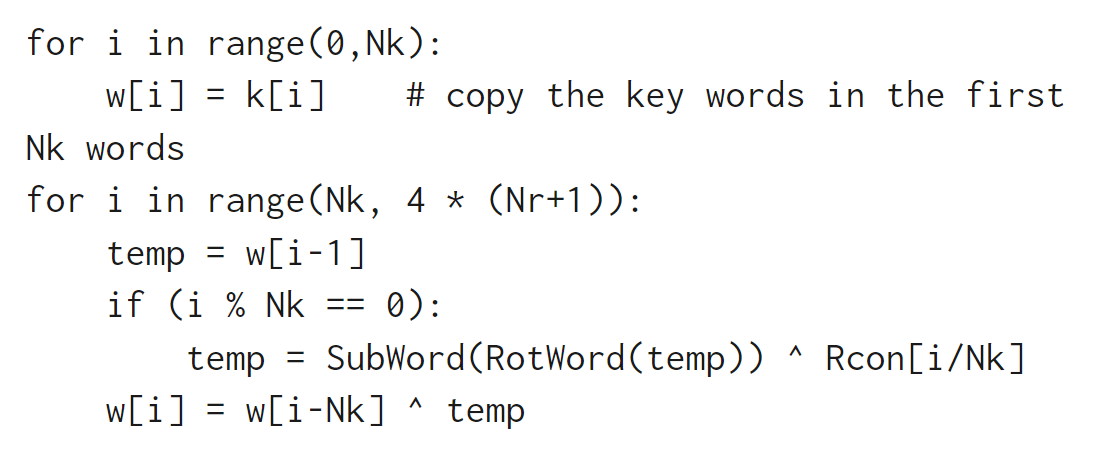
\includegraphics[scale = 0.8]{img/aes9.png}
        \label{aes9}
        \caption{Key Expansion operation}
    \end{figure}

    IMPORTANT NOTE: for 256 bit key, when i-4 is a multiple of $N_k$ \textit{SubWord} is applied to $w[i-1]$ before the XOR. This has been omitted in the code for the sake of readability. Moreover, note that of course the first byte of \textit{Rcon} can be precomputed.

\end{enumerate}

Here is the \textbf{overall scheme} for AES assuming that variable state is initialized with the 4x4 matrix of the plaintext (see above) and $w[]$ has been initialized by key expansion.

\imageLabel{img/aes10.png}{0.8}{Scheme of AES - Encryption}{aes10}

Notice that in the \textbf{last round we do not perform} the \textit{MixColumn} \textbf{operation}.

\textbf{Decryption} is computed by \textbf{applying inverse operations}.

\imageLabel{img/aes11.png}{0.8}{Scheme of AES - Decryption}{aes11}

Notice that:

\begin{enumerate}
    \item \textit{AddRoundKey} is unchanged since XOR is the inverse of itself;
    \item \textit{InvShiftRows} trivially amounts to revert the shifts on the row (to the right instead of left);
    \item \textit{InvSubBytes} is computed by using the following inverse substitution of the S-Box:

    \imageLabel{img/aes12.png}{0.8}{Inverse S-Box}{aes12}

    \item Finally, \textit{InvMixColumns} is given by the following operation:

    \imageB{img/aes13.png}{0.8}

    For example the first byte of each column is computed as $0e c_0 \oplus 0b c_1 \oplus 0d c_2 \oplus 09 c_3$.

    \textbf{NOTE}: this fixed matrix is obtained by considering each column as a four-term polynomial with coefficients in $\mathbf{GF}(2^8)$. The columns are then multiplied modulo $x^4 + 1$ with the inverse of the fixed polynomial $a(x)$, given by $a^{-1}(x) = 0b x^3 + 0d x^2 + 09 x + 0e$.
    
\end{enumerate}

The algorithm for decryption is written in a form similar to the one for encryption but operations are not in the same order. It can, in fact, become the very same algorithm by noticing that:

\begin{enumerate}
    \item \textit{SubBytes} and \textit{ShiftRows} commute. It does not matter if we first apply the byte-wise substitution or if we first shift the rows. The final result will be the same. Of course, the same holds for the inverse transformations;

    \item \textit{InvMixColumns}$(\text{state} \oplus \text{roundKey})$ = \textit{InvMixColumns}(\textit{state}) $\oplus$ \textit{InvMixColumns}(\textit{roundKey}). This allows for inverting the two functions, provided that \textit{InvMixColumns} is applied to the all the round keys.

\end{enumerate}

Call $dw$ the array containing the round keys transformed via InvMixColumns. The final decryption algorithm is represented in Picture \ref{aes16}.

\imageLabel{img/aes16.png}{0.8}{Decryption algorithm}{aes16}

This is exactly the same as the one for encryption, but with the inverse functions. Having the same algorithm for encryption and decryption simplifies a lot implementations, especially if they are done in hardware.

The final scheme of the AES algorithm is provided in Picture \ref{aes14}: note that AES is a symmetric key algorithm.

\imageLabel{img/aes14.png}{0.8}{AES algorithm}{aes14}

Finally, we recall the fact that the security of AES depends on the number of rounds that are executed: the more rounds, the more secure the algorithm is.

\subsection{Block cipher modes of operation}
When using block ciphers we have to face the problem of encrypting \textbf{plaintexts} that are \textbf{longer} than the \textbf{block size}. We then adopt a \textbf{mode of operation}, i.e., a \textbf{scheme} that repeatedly applies the \textbf{block cipher} and allows for encrypting a plaintext of arbitrary size.

\subsubsection{Electronic CodeBlock mode (ECB)}
This is the simplest mode and is, in fact, what we have done so far with classic ciphers: the \textbf{plaintext} $X$ is split into \textbf{blocks} $x_1,x_2,\ldots,x_n$ whose \textbf{size} is exactly the same as the size of the \textbf{cipher block}. Each \textbf{block} is then \textbf{encrypted} independently using the fixed \textbf{key} $k$. For example, a substitution cipher applies to letters. What we do is to split the plaintext into single letters that are encrypted independently.

\image{img/bcm1.png}{0.90}{ECB: Encryption}

\textbf{Decryption} is done, as expected, by reversing the scheme:

\image{img/bcm2.png}{0.90}{ECB: Decryption}

\underline{\textbf{Advantage}}: this scheme has the advantage of being very \textbf{simple} and \textbf{fast}, especially on \textbf{multi-core computers}. Notice, in fact, that each single encryption/decryption can be performed \textbf{independently}.

\underline{\textbf{Disadvantages}}: the \textbf{security} of the scheme, however, is \textbf{poor}. Indeed:

\begin{enumerate}
    \item It mainly conveys all the \textbf{defects} of \textbf{monoalphabetic classic ciphers}: equal plaintext blocks are encrypted in the same way. This allows for the construction of a code-book (from which the mode name) mapping ciphertexts back to plaintexts. It is often the case, in practice, that part of a plaintext is fixed due to the message format, for example. Think of a mail starting with “Dear Alice, …”. If we know a part of the plaintext, we know how the blocks containing that part are encrypted. We can use this information to decrypt other parts of the message, whenever we see the same block occurring.

    Picture \ref{bcm5} provides an immediate visualization of the codebook problem described above.

    \imageLabel{img/bcm5.png}{0.8}{Attack on ECB}{bcm5}

    \item Another crucial limitation of this mode is the complete \textbf{absence of integrity}: an \textbf{attacker} in the middle might duplicate, swap, eliminate encrypted blocks and this would correspond to a plaintext where the same blocks are duplicated, swapped, eliminated. Again, having information about the format of the plaintext, an attacker might be able to obtain a different meaningful plaintext. How critical is this attack really depends on the application. But it is not a good idea to leave such an easy opportunity.
    
\end{enumerate}

\subsubsection{Cipher Block Chaining mode (CBC)}
This mode solves or mitigates all the issues of ECB discussed above: it \textbf{prevents} \textbf{equal plaintexts} to be \textbf{encrypted} the \textbf{same way} and, at the same time, it provides a \textbf{higher degree of integrity}, even if it is not yet satisfactory on this aspect. The idea is to \textbf{“chain” encryption of blocks} using the \textbf{previous encrypted block}. The first block is chained with a special number called \textit{Initialization Vector} (\textit{IV}) that is kept secret together with key $k$.

\image{img/bcm3.png}{0.90}{CBC: Encryption}

\textbf{Decryption} is as follows:

\image{img/bcm4.png}{0.90}{CBC: Decryption}

\underline{\textbf{Advantage}}: as mentioned above, \textbf{CBC} \textbf{never encrypts the same plaintext block in the same way}, preventing the code-book attack. \textbf{Integrity} is improved, but is not yet completely satisfactory. If an attacker swaps, duplicates or eliminates encrypted blocks this will result in at least one corrupted plaintext block. Notice however that this might be unnoticed at the application level and, again, we cannot leave to the application the whole task of checking integrity of decrypted messages.

\underline{\textbf{Disadvantage}}: using \textbf{XOR} introduces a \textbf{new weakness}: the \textbf{attacker} manipulating \textbf{one bit} of an \textbf{encrypted block} $y_i$ obtains that the \textbf{same bit of plaintext} $x_{i+1}$ is also \textbf{manipulated}. At the same time $x_i$ is corrupted.

\subsubsection{Output FeedBack mode (OFB)}
We now see two modes of operation that “transform” block ciphers into stream ciphers. The general idea is to use the block cipher to generate a complex key stream. Encryption is then performed by just XOR-ing the plaintext blocks with the keys of the stream. Intuitively, this is like one-time-pad with a generated key stream. The more the stream is close to a random stream the more the cipher will be close to a perfect one.

\image{img/bcm6.png}{0.90}{OFB: Encryption}

Notice that key generation is completely independent of the plaintext and ciphertext. In fact, it is possible to generate the key stream offline, having key k, and perform encryption later on, when necessary. Decryption simply consists of “swapping the arrows” when performing the XOR: ciphertexts are XOR-ed with the key stream to recover the plaintexts.

\image{img/bcm7.png}{0.90}{OFB: Decryption}

Notice that the generation of the key stream is, in fact, CBC encryption of a zero plaintext (indeed, notice that in this case we do not have the top level $x_i$ XOR $y_{i-1}$). It is thus possible to reuse CBC implementations to compute it. Notice also that the plaintext blocks can be smaller that the size of the block cipher. In that case it is possible to use part of the key and use the remaining part for the next block. For example, if the size of the block is 128 bits (like in AES), and we have to encrypt single bytes we have that one key can be split into $128/8 = 16$ keys of 8 bits, each used to encrypt a single byte.

\underline{\textbf{Advantages}} 

\begin{itemize}
    \item This cipher is very efficient (key can be precomputed using CBC) and allows for the encryption of streams of plaintexts;
    \item Key stream is generated through a block cipher which makes it very hard to be predicted;
    \item Finally, notice that it works very well when IV changes every time we encrypt a new block.
\end{itemize}

\underline{\textbf{Disdvantages}} 

\begin{itemize}
    \item This stream cipher is synchronous since the key stream is independent of the plaintext. As a consequence, if we reuse the same IV with the same key we obtain the same key stream. Since encryption is XOR, attacking the cipher is the same as attacking one-time-pad when the key is used more than once. Thus, the IV must be changed any time we encrypt a new message under the same key k;
    \item Moreover, an attacker in the middle can arbitrarily manipulate bits of the plaintext by swapping the corresponding bits in the ciphertext. No decrypted blocks will be corrupted. For this reason this mode should only be used in application where integrity of the exchanged message is not an issue or is achieved via additional mechanisms. An example could be satellite transmissions where an attacker is extremely unlikely to be in the middle and confidentiality is the only issue. In this setting, absence of integrity becomes useful to avoid noise propagation: an error on one bit will only affect one bit of the plaintext.
\end{itemize}

\underline{NOTE}: there exists a variation of OFB, called \textbf{Counter mode} (\textbf{CTR}), where IV is a random number (nounce) and a counter. The random number can be sent in clear (the bit should change and any new stream generation), and the counter changes the value during the stream generation. This mode is widely used in practice.

\image{img/bcm10.png}{1.8}{CTR: Encryption}

\subsubsection{Cipher FeedBack mode (CFB)}
This mode mitigates the problems of OFB by making the key stream dependent on the previous encrypted element. To preserve the ability of encrypting plaintexts of size less than or equal to the size of the block of the cipher (e.g. a single byte), this mode uses a shift register that is updated at each step: the register is shifted to the left the number of bits of previous ciphertext (8 for a byte), and such a ciphertext is copied into the rightmost bits of the register.

\image{img/bcm8.png}{0.90}{CFB: Encryption}

In this sense, in the first phase we use IV, and in the following ones we use blocks of the previous outputs ($\text{IV}|y_1$ or $y_{n-2}|y_{n-1}$). Decryption is as follows:

\image{img/bcm9.png}{0.90}{CFB: Decryption}

As for OFB, the key stream is generated and then XOR-ed to the ciphertexts to reconstruct the plaintexts.

\underline{\textbf{Advantage}}: this mode provides a higher degree of integrity with respect to OFB: whenever one bit of one ciphertext is modified, the next BSize/CSize plaintexts are corrupted, where BSize is the size of the block of the cipher (e.g., 128 bites) and CSize is the size of the single ciphertext (e.g., 8 bits). For example, with AES and 8 bits of plaintext/ciphertext sizes, we have $128/8 = 16$ corrupted decryptions. This number corresponds to the number of left shifts necessary for a ciphertext to exit the shift register. 

\underline{\textbf{Disadvantage}}: on the other hand, this cipher is slower than OFB as it requires the previous ciphertext to compute the next, meaning that parallelization is impossible when encrypting. Moreover, for noisy transmissions (e.g., satellite, TV, ..) it has the problem of propagating an error on a single bit over the next BSize/CSize plaintexts, which are completely corrupted.

\subsection{More block ciphers}
There are many other ciphers in use, in addition to AES. We list some here giving a very brief summary of their features.

\subsubsection{Data Encryption Standard (DES)}
This is the predecessor of AES. It has been published in 1975 and derives from Lucifer (IBM). It has been the most used and implemented cipher in the history and it is currently used in many application, especially in the triple version below (this version uses 3 keys of 56 bits, which make it invulnerable to brute force attacks). 

DES major problem is the key-length (only 56 bits) that is considered vulnerable with modern parallel computers. Indeed, notice that this key length ony generates $2^{56}$ possible keys, so it is prone to brute force attacks. There are also some analytical results which demonstrate theoretical weaknesses in the cipher, although they are infeasible to mount in practice.

\paragraph{Operations}

The DES cipher takes a fixed-length string of plaintext bits and transforms it through a series of complicated operations into another ciphertext bit string of the same length. We have that:

\begin{itemize}
    \item The block size is 64 bits;
    \item Key is of 56 bits (8 for error correction)
\end{itemize}

The operations are the following:

\begin{itemize}
    \item 16 identical rounds;
    \item Initial permutation (IP) and final permutation (FP, inverse operation);
    \item Before the main rounds, the block is divided into two 32-bit halves and processed alternately:

    \begin{itemize}
        \item The first half is XOR-ed with the result of F, and the result is given as input to the F of the following round;
        \item The second half is provided as input to the F function, and it is also XOR-ed with the result of the F function of the following round.
    \end{itemize}
\end{itemize}

\image{img/des1.png}{0.90}{DES: operations}

\paragraph{Feistel function}

This function is composed of the following operations:

\begin{enumerate}
    \item E: permutation and expansion (from 32 to 48 bits);
    \item Key-mixing (key schedule), where the 48 bits are XOR-ed with a subkey of 48 bits, extracted from the original key (56 bits) using permutation and circular shifts;
    \item Substitution using S-box, and compression (results 32 bits). In this case, from 8 blocks of 6 bits we retrieve 8 blocks of 4 bits;
    \item P: permutation.
\end{enumerate}

\image{img/des2.png}{0.60}{F function}

The result of the F function is a 32-bit information, which is consistent with the previous schema, since it is XOR-ed with half of the original block of 64 bits. The alternation of substitution from the S-boxes, and permutation of bits from the P-box and E-expansion provides so-called "confusion and diffusion” (Shannon).

\paragraph{Confusion and diffusion}

\begin{itemize}
    \item Confusion: the process drastically changes data from the input to the output (e.g., by translating data through a non-linear table created from the key);
    \item Diffusion: changing a single character of the input will change many characters of the output.
\end{itemize}

\subsubsection{International Data Encryption Algorithm (IDEA)}
This cipher was proposed in 1990 as a substitute of DES. It is currently adopted in many applications. 

This cipher is not based on non-linear substitutions (S-Boxes); instead, confusion and diffusion are obtained by a combination of three operations: XOR, sum and multiplication modulo 216. Patent issues have reduced the popularity of this cipher. Compared to other, IDEA performance is not so high.

\subsubsection{Blowfish and Twofish }
Blowfish has been proposed in 1993. It is a cipher with peculiar features: it is very fast, compact and simple to implement, with a very highly configurable security: key length is variable up to 448 bits which allows for security/speed trade-off. As DES it is based on XOR and S-Boxes which are not fixed but computed using the cipher itself and the actual key. These key-dependent S-Boxes make brute-forcing particularly expensive: for each key it is necessary to generate the S-Boxes which takes 522 iterations of the algorithm.

Twofish is one of the finalists of AES and is the “successor” of Blowfish. Both ciphers have been developed by Bruce Schneier.

\subsubsection{RC2, RC5, RC6}
This is a family of ciphers developed by Ron Rivest (one of the fathers for RSA public-key cipher). RC5 (1994) has the peculiar feature of using data dependent rotations. Moreover, the cipher is extremely simple but requires a complex key-expansion procedure: each round is just two XORs, two sums modulo and two rotations. This cipher is highly configurable on the number of rounds, key-length and word-length, which allows for a sophisticate trade-off between security and performance.
RC6 has been one of the AES finalists.

\subsection{Meet-in-the-middle attack - 3DES}
One technique to strengthen ciphers is iteration. We have seen that all modern ciphers are based on rounds, i.e., repetitions of the same core algorithm. We might wonder what happens if we iterate a whole cipher such as DES or AES. There is at least a good reason for that: increasing key length. DES, for example, has a 56-bit key that is considered weak nowadays. If we iterate the cipher using a different key we obtain a key pair (k1,k2) of 112 bits which is, in principle, too hard to break (but we will see that this is not the case).

\subsubsection{3DES}
It is a triple iteration of DES. The aim is to increase the key-length. Due to the meet-in-the-middle attack, the triple key of 168 bits is, in fact, equivalent in strength to a key of 112 bits. Meet-in-the-middle is also the reason why 2DES makes no sense: the 112-bit key could be broken in a 256  time/space complexity brute force attack. 3DES is implemented, for example, in SSH, TLS/SSL and is adopted in many commercial applications. Moreover, bank circuits and credit card issuers use it in smartcard based applications and for PIN protection.

\paragraph{DES is non-idempotent}
We know that iteration makes sense only if the cipher is not idempotent, otherwise the result of its composition would be the same cipher, so it would be useless. The following informal argument suggests that modern ciphers are very unlikely to be idempotent. We reason on DES but the same reasoning would apply to different block ciphers.

DES has a block size of 64 bits. If we list all the $2^{64}$ possible blocks and we pick one DES key, the cipher will map each of these blocks into a different block. Since encryption must be invertible, this mapping is injective. Thus, in any block cipher, a key corresponds to a permutation of all the possible plaintext blocks.

\imageB{img/des3.png}{0.60}

So, for example, 0 (64 zero bits) is mapped to 3214112, 1 to 213210312421 and so on. 

Now, the number of permutations of $2^{64}$ elements is $2^{64}!$ which is enormously big compared to the $2^{56}$ DES keys. We reason as follows: the way a DES key selects a specific permutation is “complex” (otherwise the cipher would be weak). We can thus think of DES keys as selecting a random subset of $2^{56}$ permutations among the $2^{64}!$ possible ones. Now, the probability that the composition of two such permutations is still in this subset is, intuitively, $2^{56} / 2^{64}!$ which is a very small, negligible number. This means that it is really unlikely that 2 iterations of DES (and of any modern block cipher, in fact) correspond to a single encryption under a different key.

As far as DES is concerned, it has been formally proved that it is not idempotent.

\paragraph{Meet-in-the-middle}
We thus consider DoubleDES (2DES), i.e., the iteration of DES twice.

\textit{Is it really true that now, in order to break the cipher, we have to try all the possible key pairs?}

The answer is ‘NO’. We can do better by exploiting the so called Meet-in-the-middle attack. It is a known-plaintext scenario, i.e., the attacker knows pair of plaintext/ciphertext $(X,Y), (X’,Y’), (X'',Y''), ..$ all encrypted under the same key $K$. The idea is:

\begin{enumerate}
    \item Select one pair, say $(X,Y)$, and try to decrypt $Y$ with all the possible second keys $k2$;
    \item All the resulting values $Z$ are stored into a table together with the key, which is indexed by $Z$;
    \item Now we try to encrypt under all the possible first keys $k1$ the plaintext $X$ and we look the obtained value into the table. If we find a match we test the resulting pair $(k1,k2)$ on all the other plaintext/ciphertext pairs and, if all the tests succeeds, we give it as output.
\end{enumerate}

The attack is illustrated below:

\imageB{img/des4.png}{0.50}

The computational cost of this attack is $2^{57}$ steps and $2^{56}$ space. In fact, first step takes $2^{56}$ steps to build a table which is $2^{56}$ entries. Second step takes at most $2^{56}$ steps to find the right key. We thus have $2^{56}$ + $2^{56}$ = $2^{57}$ steps.

\paragraph{False keys}

It is very important that, whenever a pair $(k1,k2)$ for $(X,Y)$ is found, it is tested against other pairs $(X’,Y’)$. It could be the case, in fact, that a key pair is fine for $(X,Y)$ but it is not the right key pair. This can happen more frequently than expected. 

To estimate the number of these false keys we assume that plaintexts are mapped to ciphertext uniformly by the possible keys. In other words, the number of keys mapping $X$ into $Y$ is approximatively the same as the number of keys mapping $X$ into any other ciphertext $Y’$. This assumption typically holds for any good cipher for which observing $Y$ gives very little information about the plaintext $X$. Having a non-uniform distribution would imply that the plaintexts mapped by more keys into $Y$ are more likely than the ones mapped by less keys.

Under this assumption, we can then estimate the number of false keys as $|K|/|C|$, i.e., the number of keys divided by the number of ciphertexts which is, for 2DES, $2^{112}/2^{64} = 2^{48}$. This huge number of possible keys encrypting $X$ into $Y$ can be reduced very quickly by testing keys on more pairs. The probability that a false key is also OK for $(X’,Y’)$ is just 1 over the number of all the possible ciphertexts (we have only one good case $Y’$ over all the possible $2^{64}$ ciphertexts) giving $1⁄2^{64}$ (which is the result of $2^{48} * 1/2^{64}$). Thus, the number of false keys is reduced to $2^{48}⁄2^{64} = 1⁄2^{16}$. If we try on one more pair we get $1⁄2^{80}$, and so on. In summary, with 3 available pairs of plaintext/ciphertext we can run the attack having a negligible probability of getting a false key.

\subsubsection{Recap}
The cost in time is thus basically the same as the one for a single iteration of DES. For this reason, 2DES is never used in practice and, instead, we have a triple iteration known as triple-DES (3DES). This gives a 168-bit triple key $(k1,k2,k3)$. The meet-in-the-middle attack is still possible but it reduces the cost in time to 2112 with a table of size 256 entries. The idea is to build the table by decrypting $Y$ under all $k3$ and then try all the pairs $(k1,k2)$, as illustrated below.

\imageB{img/des5.png}{0.50}

\subsection{Asymmetric-key ciphers}
All the ciphers we have studied so far use the \textbf{same key} $K$ both for \textbf{encryption} and \textbf{decryption}. This implies that the source and the destination of the encrypted data have to \textbf{share} $K$. For this reason, this kind of ciphers are also known as \textbf{symmetric-key ciphers}. This aspect becomes \textbf{problematic} if we want cryptography to \textbf{scale} to big systems with many users willing to communicate securely. Unless we have a centralized service to handle keys (that we will discuss later), for $N$ users this would require $N(N-1)/2$, i.e., $O(N^2)$, keys. For example, for a LAN with 1000 users we would have $\approx 500000$ keys. These keys should be pre-distributed to users in a secure way (e.g., offline). This is totally \textbf{impractical} and would never scale on a wide-area network such as the Internet.

The above argument has been one of the main motivation leading to the \textbf{development} of \textbf{asymmetric-key cryptography}. In \textbf{1976} Diffie and Hellman suggested the existence of this revolutionary ciphers, which are based on the idea that a user $A$ has one \textbf{encrypting} and one \textbf{decrypting} \textbf{key}, which are \textbf{different} but \textbf{correlated} (this is why they are called asymmetric). The characteristic is that the \textbf{encrypting key} is \textbf{public}, while the \textbf{decrypting key} is a \textbf{secret} known only by $A$. In this sense, for $N$ users we have $N$ \textbf{public} keys, which are used for \textbf{encryption}, and $N$ \textbf{private} keys, which are used for \textbf{decryption}. The public key is published in a public list and is known by everybody, even the attacker, and they are correlated with private keys, but the knowledge of the public key does not give any information about the private key.

\subsubsection{Definition}
Intuitively, if we denote with $PK_A$ the public key of $A$ and with $SK_A$ the secret key of $A$, then:

\begin{itemize}
    \item $B$ sends an encrypted message $E_{PK_A}(M)$ to $A$;
    \item $A$ receives it and decrypts it as $D_{SK_A}(E_{PK_A}(M))=M$.
\end{itemize}

Moreover, encryption and decryption algorithms are such that

$$D_{SK_A}(E_{PK_A}(M))=M$$

holds. We can notice that any user can perform the encryption $E_{PK_A}$, so our goal is to define a decryption function that is unfeasible to broke, otherwise the cipher would be useless.

More formally, an asymmetric-key cipher is a \textbf{quintuple} $({\cal P},{\cal C},{\cal K}_S\times{\cal K}_P,E,D)$ with $E : {\cal K}_P \times {\cal P} \rightarrow {\cal C}$ and $D : {\cal K}_S \times {\cal C} \rightarrow {\cal P}$ (\textit{which was the tuple for symmetric ciphers?}) and such that:

\begin{enumerate}
    \item It is \textbf{computationally easy} to generate a \textbf{key-pair} $(SK, PK) \in{\cal K}_S\times{\cal K}_P$;
    \item It is \textbf{computationally easy} to compute $y = E_{PK}(x)$;
    \item It is \textbf{computationally easy} to compute $x = D_{SK}(y)$;
    \item \textbf{Decryption} under $SK$ of a plaintext $x$ \textbf{encrypted} under $PK$ gives the initial \textbf{plaintext} $x$. Formally, $D_{SK}(E_{PK}(x)) = x$;
    \item It is \textbf{computationally infeasible} to compute $SK$ knowing $PK$ and $y$;
    \item It is \textbf{computationally infeasible} to compute $D_{SK}(y)$ knowing $PK$ and $y$ and without knowing $SK$;
\end{enumerate}

Intuitively, instead of one key we now have a \textbf{key pair} $(SK,PK)$ composed of a \textbf{private} and a \textbf{public} key, respectively. \textbf{Encryption} is performed under $PK$ while \textbf{decryption} under $SK$. Thus, \textbf{decryption key} is now \textbf{different} from \textbf{encryption key}. 

Items 1,2 and 3 state that it should be \textbf{practical} to \textbf{generate key pairs} and to encrypt/decrypt data. 

Item 4 states that \textbf{decrypting} under the \textbf{private key} a \textbf{plaintext} \textbf{encrypted} under the \textbf{public key} gives the initial \textbf{plaintext}.

Items 5 and 6 state that the \textbf{cipher} should be \textbf{secure} regardless of the secrecy of the public key $PK$.  This is the \textbf{main challenge} behind this kind of cryptography: the \textbf{public} and the \textbf{private} key have to be \textbf{related}, otherwise decryption would never work, but, at the same time, \textbf{computing} the \textbf{private key} from the public key should be \textbf{impossible} in practice (computationally infeasible).

\subsubsection{Security properties}
What security properties do we have?

\begin{itemize}
    \item \textbf{Secrecy}: this property clearly holds, since we're taking into consideration a cipher;
    \item \textbf{Authentication}: this property does not hold, since the receiver cannot retrieve the identity of the sender, because the key for encryption is public, i.e. known to everybody. Thus, in this case to ensure this property we would also need a digital signature.
\end{itemize}

Notice that in the case of symmetric cipher, both the properties hold, since in that case each sender/receiver share a single key, so the authenticity is ensured.

\subsubsection{One-way trap-door functions}
\textbf{Asymmetric-key ciphers} are strictly \textbf{related} to \textbf{one-way trap-door functions}.

\textbf{Definition.} An \textbf{injective}, \textbf{invertible} \textbf{function} $f$ is \textbf{one-way}, if and only if:

\begin{enumerate}
    \item $y = f(x)$ is \textbf{easy} to compute (i.e. encryption is computationally easy);
    \item $x = f^{-1}(y)$ is \textbf{infeasible} to compute (i.e. decryption is computationally hard).
\end{enumerate}

Note that one-way does not refer to the fact the function does not admit an inverse.: \textbf{one-way} functions are \textbf{invertible} but \textbf{computing their inverse} is too \textbf{expensive} to be feasible in practice.

\textbf{Definition.} An \textbf{injective}, \textbf{invertible} \textbf{family of functions} $f_K$ is \textbf{one-way trap-door}, if and only if, given $K$, we have that:

\begin{enumerate}
    \item $y = f_K(x)$ is \textbf{easy} to compute;
    \item $x = f^{-1}_K(y)$ is \textbf{infeasible} to compute \textbf{without knowing the secret trap-door} $S(K)$ relative to $K$.
\end{enumerate}

Thus, intuitively, the trap-door is a hidden way to go back to the pre-image $x$ of the function: \textbf{only knowing the trap-door we can compute the inverse} of $f_K$.

\subsubsection{The Merkle-Hellman knapsack system}
We present now an example cipher that has been broken, but still gives a very immediate idea of how asymmetric-key ciphers relate to one-way trap-door functions. The cipher is based on the following NP-complete problem.

\paragraph{The subset-sum problem} 
Let $s_1, .., s_n$ and $T$ be positive integers: $s_i$ are \textbf{sizes} while $T$ is the \textbf{target}. A \textbf{solution} to the subset-sum problem is a \textbf{subset} of $(s_1, .., s_n)$ whose \textbf{sum} is exactly the \textbf{target} $T$. 

Formally, the solution is a binary tuple $(x_1, .., x_n)$ such that $\sf\sum_{i=1}^{n}{} x_i s_i = T$.


For example, if sizes are $(4,6,3,8,1)$ and $T=11$, we have that $(0,0,1,1,0)$ and $(1,1,0,0,1)$ are solutions, since $3+8 = 11$ and $4+6+1 = 11$.

This \textbf{problem} is \textbf{NP-complete} in general. As a consequence, we can easily obtain a one-way function from it. Notice, in fact, that NP problems have a non-deterministic polynomial solution meaning that checking if a solution is correct can be done in polynomial time. If we define $f(x_1, .., x_n) = \sf\sum_{i=1}^{n}{} x_i s_i$, we have that $f$ is clearly easy to compute but \textbf{inverting} this function amounts to \textbf{finding} $(x_1, .., x_n)$ from a \textbf{target} $T$ which we know to be \textbf{infeasible} for a big $n$.

How can we now introduce a secret trap-door to allow us inverting the function? The trick is to start from a specific instance of the problem that is easy to solve. We consider special \textbf{sizes} that are \textbf{super-increasing}, i.e., such that $\sf s_i > \sum_{j=1}^{i-1} s_j$, for each $i>1$. Intuitively, any $s_i$ is bigger than the sum of all the previous $s_j$. For example (1,3,5,10) is super-increasing while (1,3,5,9) is not. In this special case there is a very \textbf{efficient algorithm} to solve the \textbf{subset-sum problem}. The idea is to \textbf{start} from the \textbf{biggest element} $s_n$ and go back to the first one: if $s_i$ fits into $T$ we pick it (we set $x_i=1$) and we subtract $s_i$ from $T$. Python example code follows.

\image{img/asy1}{0.5}{Solution of the subset-sum problem with super-increasing sizes}

\example{\text{subsetSum}($[1,3,5,10]$, 11) returns $[1, 0, 0, 1]$, while \text{subsetSum}($[1,3,5,10]$, 12) returns the empty list $[]$, since there's no solution in this case.}

\paragraph{The cipher}
We now proceed as follows:

\begin{enumerate}
    \item We start from a \textbf{super-increasing} problem $(s_1,\ldots,s_n)$;
    \item We choose a \textbf{prime} $p > \sum_{i=1}^{n}{s_i}$;
    \item We choose a \textbf{random} $a$ such that $1 < a < p$;
    \item We \textbf{transform} the initial super-increasing problem into $(\hat{s_1}, \ldots, \hat{s_n})$, with $\hat{s_i} = a s_i \mod p$. Notice that \textbf{this problem} is \textbf{not super-increasing in general};
\end{enumerate}

The \textbf{trap-door} is composed of the \textbf{initial problem} and values $p$ and $a$, that are kept \textbf{secret}. Intuitively, \textbf{encryption} is done by \textbf{computing the target} for the \textbf{problem} $(\hat{s_1}, \ldots, \hat{s_n})$. Since this is not super-increasing, finding the initial plaintext $x_1, \ldots, x_n$ is \textbf{infeasible} (for a big $n$). However, \textbf{knowing} the \textbf{secret trap-door} we can \textbf{derive} from the \textbf{ciphertext} a \textbf{target} for the initial easy super-increasing problem, and then solve it using the efficient algorithm above. 

More precisely, \textbf{encryption} and \textbf{decryption} are defined as follows:

\begin{itemize}
    \item $E_{PK}(x_1, \ldots, x_n) = \sum_{i=1}^{n}{x_i \hat{s_i}}$;
    \item $D_{SK}(y)$ is the solution of the super-increasing problem $(s_1,\ldots,s_n)$ with target $a^{-1} y \mod p$.
\end{itemize}

Notice that $a^{-1} \mod p$ is guaranteed to \textbf{exist} by the fact $p$ is a \textbf{prime} number. We will prove this in the next lesson. 

The \textbf{correctness} of the above cipher can be proved as follows:

$$\begin{array}{rcl}E_{PK}(x_1, \ldots, x_n) &=& \sum_{i=1}^{n}{x_i \hat{s_i}}\\ & = & \sum_{i=1}^{n}{a x_i  s_i \mod p}\\& = & a\sum_{i=1}^{n}{x_i  s_i \mod p}\end{array}$$


, thus

$$\begin{array}{rcl}a^{-1}E_{PK}(x_1, \ldots, x_n) \mod p &=& a^{-1} a\sum_{i=1}^{n}{x_i  s_i \mod p}\\ &=& \sum_{i=1}^{n}{x_i  s_i \mod p}\\ &=& \sum_{i=1}^{n}{x_i  s_i}\\\end{array}$$

, since we have that $p > \sum_{i = 1}^n s_i$ by construction. 

The previous equations show that the \textbf{transformed target} $a^{-1} y \mod p$ is, in fact, the \textbf{target} for the \textbf{initial}, easy \textbf{problem}.

\example{Let $(1,2,5,12)$ be a super-increasing problem. We let $p=23$ and $a=6$. We have that $a^{-1} = 4$, since $6 \cdot 4 \mod 23 = 1$. If we compute $s_i \cdot a \mod p$ we obtain $(6,12,7,3)$ which is not super-increasing. Consider now the plaintext $(1,0,0,1)$. We have that $E_{PK}(1,0,0,1) = 6 + 3 = 9$. Now to decrypt we have to compute $a^{-1} \cdot 9 \mod p = 36 \mod 23 = 13$. We finally solve $(1,2,5,12)$ with target 13, which gives the initial plaintext $(1,0,0,1)$.}

\newpage
\subsection{The RSA cipher}
RSA is the most famous \textbf{asymmetric-key cipher}. It is based on a few technical results from number theory that we recall below.

\subsubsection{Background}

\paragraph{The Euler function} The Euler function $\Phi(n)$ returns the number of numbers less than or equal to $n$ that are coprime to $n$. Recall that $i$ and $n$ are coprime iff $gcd(i,n) = 1$, i.e., if the only common divisor is 1. So, for example, we have that $\Phi(3) = 2$ since 1 and 2 are coprime to 3, $\Phi(4) = 2$ since only 1 and 3 are coprime to 4 and so on. We report some values below:

$$\begin{array}{c|c}n & \Phi(n) \\ \hline 1 & 1\\2 & 1\\3 & 2\\4 & 2\\ 5&4\\ 6&2 \\ 7&6 \\ \end{array}$$

We immediately notice that if $n$ is prime then $\Phi(n) = n-1$. In fact, by definition, a prime number $n$ is coprime to all the numbers smaller than $n$. 

There is another situation where $\Phi(n)$ is easy to compute: when $n=p_1 \ldots p_k$ with $p_1 \neq p_2 \neq \ldots \neq p_k$ prime numbers, i.e. multiplication between prime numbers, we have that $\Phi(n) = \Phi(p_1) \ldots \Phi(p_k) = (p_1-1) \ldots (p_k-1)$.

\example{Consider $15 = 3 \cdot 5$, then $\phi(15) = \phi(3) \cdot \phi(5) = 2 \cdot 4 = 8$.} 

We prove this result for $n = pq$ with $p\neq q$ primes (i.e. we want to prove that $\phi(n) = \phi(p) \phi(q) = (p-1)(q-1)$). The numbers less than $n$ that are not coprime to $n$ is exactly the multiples of $p$ and $q$, i.e., $p,2p,\ldots,(q-1)p,q,2q,\ldots,(p-1)q$ that are $(q-1)+(p-1)$. Now we have that $\Phi(n) = pq-1 - (q-1)-(p-1) = pq -q -p +1  = (p-1)(q-1)$.

\example{Consider $14 = 2 \cdot 7$. Then, $\phi(14) = 13 - 6 - 1 = 6$, where 6 is the number of multiples of 2 up to 14, while 1 is the only multiple of 7 up to 14.}

\theoremName{Euler theorem}{Let $a$ and $n$ be coprime, i.e., $\text{gcd}(a,n)=1$. Then $$a^{\Phi(n)} \mod n = 1$$}

\textit{Proof.} Let $S = (s_1, \ldots, s_{\Phi(n)})$ be the $\Phi(n)$ numbers less than $n$ and coprime with $n$. We consider $R = (a s_1 \mod n, \ldots, a s_{\Phi(n)} \mod n)$ and we show that $S = R$. We need a few lemmas:

\lemma{1}{Let $x,y$ be coprime to $n$. Then $xy$ is coprime to $n$.}

\textit{Proof.} This can be easily proved by considering that all divisors of $xy$ are products of divisors of $x$ or $y$. Thus a common divisor of $xy$ and $n$ must also divide $x$ and/or $y$. Thus, $\text{gcd}(xy,n)>1$ would imply that $\text{gcd}(x,n)>1$ or $\text{gcd}(y,n)>1$ giving a contradiction.

\example{Let $x = 7$, $y = 3$, $p = 5$ and $q = 11$. Then $n = 55$, $x$ and $y$ are coprime to 55, what about $xy = 21$? We have that $\text{gcd}(21,55) = \text{gcd}(7*3, 5*11) = 1$}.

\lemma{2}{Let $x$ be coprime to $n$. Then $x \mod n$ is coprime to $n$.}

\textit{Proof.} Since $x \mod n = x - kn$ we have that any common divisor $d$ of $x \mod n$ and $n$ must divide $x$. In fact, $\frac{x \mod n}{d} = t = \frac{x - kn}{d} = \frac{x}{d} - kr$ that implies $\frac{x}{d}$ is an integer value. That is, $d$ divides $x \mod n$, $n$ and $x$. However, if $x$ is coprime to $n$, then $x \mod n$ is coprime to $n$.

\example{Let $x = 57$, $p = 5$, $q = 11$, then $n = 55$. We have that $x = 57$ is coprime to 55, what about $x \mod n = 2$? We have that $\text{gcd}(2,55) = 1$}.

\lemma{3}{Let $ax \mod n = ay \mod n$ with $\text{gcd}(a,n)=1$. Then $x \mod n = y \mod n$.}

\textit{Proof.} We have $ax - kn = ax \mod n = ay \mod n = ay - jn$. Thus $ax - ay = wn$ that implies $\frac{ax - ay}{a} = \frac{wn}{a}$ and so $x-y = \frac{wn}{a}$ . Since $\text{gcd}(a,n)=1$ we have that $a$ must divide $w$ and so $x-y = tn$, i.e., $x \mod n = y \mod n$.

\example{Given $a = 3$ and $n = 6$, find $x$ and $y$ such that $ax \mod n = ay \mod n$ (here $gcd(a,n) = gcd(3,6) = 3 \neq 1$). We have that $x = 1$ and $y = 3$, since $1 \mod 6 = 1 \neq 3 \mod 6 = 3$.}

\example{Find $a$ coprime to $n$, and find $x$ and $y$ s.t. $ax \mod n = ay \mod n$. Let $a = 5$, which is coprime to 6, then $5x \mod 6 = 5y \mod 6$, from which we derive $x = 1$ and $y = 7$. That is $1 \mod 5 = 1 = 7 \mod 6$.}

Now, by Lemma 1 and 2 we have that all numbers in set $R$ are coprime to $n$ and smaller than $n$. Since $S$ is the set of all numbers coprime to $n$ and smaller than $n$ we obtain that $R \subseteq S$. Now, consider $a s_i \mod n$ and $a s_j \mod n$ in $R$. Since $a$ is coprime to $n$, by Lemma 3 we obtain that $a s_i \mod n = a s_j \mod n$ implies $s_i \mod n = s_j \mod n$, which gives a contradiction. Thus we have that $a s_i \mod n \neq a s_j \mod n$ for all $i$ and $j$. This proves that $R = S$.

To conclude the proof it is enough to observe that $$\prod_{i=1}^{\Phi(n)}{s_i} = \prod_{i=1}^{\Phi(n)}{a s_i \mod n} = a^{\Phi(n)}\prod_{i=1}^{\Phi(n)}{s_i \mod n}$$ Since all $s_i$ are coprime to $n$, by applying many times Lemma 3 we obtain $1 = a^{\Phi(n)} \mod n$, which is what we wanted to prove.

\example{Let $p=2$ and $q=3$: what happens if $a=3$ is not coprime to $n = 2*3 = 6$? We have that $a^{\phi(n)} \mod n = 3^{\phi(n)} \mod 6 = 3^3 \mod 6 = 3 \neq 1$. \\ We now try to find an $a$ that satisfies the theorem. We let $a = 5$ (5 is coprime to 6), then $5^{\phi(n)} \mod 6 0 5^2 \mod 6 = 1$}

\subsubsection{The cipher}
RSA stands for Rivest-Shamir-Adleman, the authors of the cipher in 1978. 

We let $n = pq$ with $p,q$ big \textbf{prime} numbers (we need a method for generating large prime numbers, we will consider an algorithm): notice that $\phi(n) = (p-1)(q-1)$. We then choose a small $a$, prime with $\phi(n)$ and smaller than $\phi(n)$. 

\example{Let $n = 3 \cdot 5$, then $\phi(n) = 2 \cdot 4 = 8$. We can choose $a = 7$.}

We compute the unique $b$ s.t. $ab \mod \phi(n) = 1$.

\example{Considering the previous example, we have that $b = 7$, since $7 \cdot 7 \mod 8 = 1$ (not a good example in this case, since $a = b$).}

The \textbf{public key} is $(b,n)$ while the \textbf{private key} (secret trapdoor) is $(a,n)$: notice that $a$ is secret, while $b$ and $n$ are known. We let ${\cal P}={\cal C} = \mathbb{Z}_n$. 

\textbf{Encryption} is defined as $$E_{PK}(x) = x^{b} \mod n$$ while \textbf{decryption} is $$D_{SK}(y) = y^{a} \mod n$$

\example{Let $p = 5$ and $q = 11$, then $n = 5 \cdot 11 = 55$ and $\phi(n) = 4 \cdot 10 = 40$. We choose $a$ coprime to 40 and smaller than 40, in this case $a = 23$. Thus, $SK = (23, 55)$. We compute the unique $b$ s.t. $ab \mod \phi(n) = 1$, in this case $b = 7$ (computed with the extended Euclidean algorithm). Thus, $PK = (7, 55)$. If we consider the encryption of $x = 2$, then $$E_{PK}(2) = 2^{7} \mod 55 = 128 \mod 55 = 18$$ , while the decryption of 18 results to be $$ D_{SK}(18) = 18^{23} \mod 55 = 2 $$}

\subsubsection{Correctness of RSA}

We now show the correctness of the cipher, i.e., that decrypting under the private key a plaintext $x$ encrypted under the public key gives $x$. Notice that, since $b = a^{-1} \mod \phi(n)$, then $ab \mod \Phi(n) = 1$ implies $ab = k\Phi(n) +1$ for some $k$. What we need to prove is that $x^{ab} \mod n = x$. In fact, if this holds we have:

$$D_{SK}(E_{PK}(x)) = (x^b)^a \mod n = x^{ab} \mod n = x$$

Notice now that $x^{ab} \mod n = x^{k\Phi(n) + 1} \mod n = (x^{\Phi(n)})^k x \mod n$. Thus, in order to prove $x^{ab} \mod n = x$ it is enough to show that $(x^{\Phi(n)})^k x \mod n = x$. This proof is split into two cases:

\begin{itemize}
    \item $gcd(x,n)=1$. In this case we know that Euler theorem holds, and we directly have that $x^{\Phi(n)} \mod n = 1$ which implies $(x^{\Phi(n)})^k \mod n = 1$, giving the thesis;
    \item $gcd(x,n)>1$. In this case, since $x<n$ we have that either $\text{gcd}(x,n)=p$ or $\text{gcd}(x,n)=q$. Without loss of generality we assume $\text{gcd}(x,n)=p$ (the proof for the other case is identical). We now have $x = jp$ for some $j$ and $\text{gdc}(x,q)=1$. Euler theorem gives $x^{\Phi(q)} \mod q = 1$, which implies $x^{\Phi(q)\Phi(p)} \mod q = x^{\Phi(n)} \mod q = 1$. This implies $(x^{\Phi(n)})^k \mod q = 1$ giving $(x^{\Phi(n)})^k = wq + 1$ for some $w$. We obtain \begin{array}{rcl} (x^{\Phi(n)})^k x \mod n &=& (wq + 1) x \mod n\\& =& (wq + 1) jp \mod n\\ &=& wqjp + x \mod n = x \text{ ,since $pq = n$ and $x = jp$}\end{array}. 
\end{itemize}

Thus, $D_{SK}(E_{PK}(x)) = x$ and the RSA cipher is correct.

\example{We prove that $x^{ab} \mod n = x$, using $p = 3$, $q = 11$ and $x = 2$. \\ In this case we have that $\phi(n) = (p-1)(q-1) = 20$, $PK = (b,n) = (3,33)$ and $SK = (a,n) = (7,33)$. Thus: $$x^{ab} \mod n = x^{7*3} \mod 33 = x^{21} \mod 33 = 2^{21} \mod 33 = 2$$}

\subsubsection{Implementation}
As we will discuss, RSA requires a big modulus $n$ of at least 1024 bits. With these sizes, implementation becomes an issue. For example a linear complexity $O(n)$, that is typically considered very good, is prohibitive as it would require at $2^{1024}$ steps. Every operation should in fact be polynomial with respect to the bit-size $k$.

We first observe that basic operations such as \textbf{sum}, \textbf{multiplication} and \textbf{division} can be performed in $O(k), O(k^2), O(k^2)$, respectively, by using simple standard algorithms (the one we use when we compute operations by hand). Reduction modulo $n$ amounts to compute a division which is, again, $O(k^2)$.

\paragraph{Exponentiation}
This operation is used both for \textbf{encryption} and \textbf{decryption}. First notice that we \textbf{cannot} implement \textbf{exponentiation} to the power of $b$ as $b$ \textbf{multiplications}. In fact, public and private exponents can be the same size as $n$. Performing $b$ multiplications would then require $k^2 2^k$ operation, i.e., $O(2^k)$ which is like brute-forcing the secret trapdoor and \textbf{infeasible} for $k \geq 1024$. We thus need to find some smarter, more efficient way to compute this operation.

There exists a much faster algorithm, known as \textbf{Square-and-Multiply}, that is based on the following observation: when we rise a number $x$ to a power of 2 such as 8, instead of performing 7 multiplications we can simply compute $((x^2)^2)^2 = xxxxxxxx$ which is just 3 multiplications. In general, if the exponent is not a power of 2, we can exploit a similar trick by performing some additional multiplications when needed. For example $x^{10}$ can be done as $((x^2)^2 x )^2 = xx \ xx \ x \ \ xx \ xx \ x$: after squaring twice we multiply the result by $x$ so that we have $x^5$. With a final square we obtain the result. In particular $x^{10}$ can be written as $(x^{5})^2$ which is $(x^{4}x)^2$ and finally $((x^2)^2) x)^2$: intuitively, if the exponent is even we divide it by 2 and we square, if it is odd we get one $x$ out (which is an additional multiplication) and we proceed as above. Dividing the exponent by 2 amounts to follow its binary representation.

For example, 10 is 1010. We start from the most significant bit. At each step we square and, only when we have a 1 we multiply by $x$. A python implementation follows:

\image{img/rsa1}{0.75}{Square-and-Multiply algorithm}

\example{We compute $2^{10}$, where $10 = 1010$ and $x = 2$. \\ Initially, we have that $r = 1$, so in the first round we compute $r = 1*1 = 1$, the bit is 1, so we update $r = r*x = 1*2 = 2$. In the second round, $r = 2*2 = 4$, and the bit is 0, so we do not update it. In the third round, $r = 4*4 = 16$ and the bit is 1, thus $r = 16 * 2 = 32$. Finally, in the last round $r = 32*32 = 1024$ and the bit is 0, so the result is $2^{10} = 1024$, which is correct.}

The \textbf{number of steps} in the worst case is $O(k^2)$ for the two multiplications, iterated $k$ times, giving $O(k^3)$. Thus for 1024 bits we can expect about 1 billion steps, which is still efficient on modern machines.

\paragraph{Inverse modulo $\phi(n)$}
This operation is necessary to compute the private exponent from the public one. Recall that RSA requires $ab \mod \Phi(n) = 1$. To find these two numbers, one technique is to choose $b$ and to compute its multiplicative inverse modulo $\Phi(n)$. This is guaranteed to exist, by the Euler theorem, when $\text{gcd}(b,\Phi(n))=1$. In this particular case, there is also an efficient algorithm to compute the inverse based on the Euclidean algorithm for computing gcd (see the exercises).

\subsubsection{Generating RSA exponents}
We can thus pick a random \textbf{public exponent} $b$ and compute its \textbf{inverse} modulo $\Phi(n)$. This works if we are lucky and $b$ is coprime to $\Phi(n)$. This happens quite frequently. It can be proved that two random numbers are coprime with probability $\approx 0.6$. Thus iterating this 2-3 times should give a suitable pair of public, private exponents.

In practice, however, it is often the case that the \textbf{public exponent} is a \textbf{fixed constant}, typically the prime number $2^{16} +1 = 65537$. Using a low exponent improves the performance of encryption (recall that each 1 in the exponent requires an extra multiplication). In this case, of course, we have to choose $n$ so that $\Phi(n) = (p-1)(q-1)$ is not a multiple of 65537.

\paragraph{RSA and factorization}
Notice that knowing $\Phi(n)$ makes it very simple to compute the private exponent. Factoring $n$ into $pq$ allows for computing $\Phi(n) = (p-1)(q-1)$. Thus we now understand that RSA security is based on the \textbf{infeasibility} of \textbf{factoring} the modulus $n$. For this reason we require $n$ to be at least 1024 bits: numbers of this size are still considered impossible to factor in a reasonable time. A size of 2048 is however already suggested for critical applications. Moreover, if we compute $\Phi(n)$ we can easily factor $n$ since we have a system of 2 equations with two variables $p,q$:

$$
\begin{cases}
    n = pq \\
    \phi(n) = (p-1)(q-1)
\end{cases}
$$

By solving it we can find $p$ and $q$. We thus have that finding $\Phi(n)$ is at least as difficult as factoring. This gives \textbf{high confidence} of the \textbf{difficulty} of breaking the private exponent by simply computing the inverse modulo $\Phi(n)$. However, there could be other ways to break the cipher. We will discuss this more in detail in the next lessons.

\subsubsection{Primality test}
We finally see how to \textbf{generate two big prime numbers}. The oldest algorithm for finding prime numbers is due to Eratosthenes and is known as the \textbf{“Sieve of Eratosthenes”}. In order to discover all prime numbers less than or equal $N$ we write all numbers from 2 to $N$. We then start from the smallest (2, initially) that we call $p$ and we remove from the list all of its multiples $2p, 3p, .. $. We iterate the procedure by picking the smallest $p$ survived from previous steps.

\example{Let $N = 10$, and we pick all the numbers from 2 to 10, i.e. $\{2,3,4,5,6,7,8,9,10\}$. Then, starting from 2, we remove 2,4,6,8,10, and we get $\{3,5,7,9\}$. Then, we take 3 and we remove 3 and 9, and we get $\{5,7\}$. Then, we take 5 and we remove 5, and we get $\{7\}$. Finally, we take 7 and we remove 7. Thus, the prime numbers between 2 and 10 are $\{2,3,5,7\}$.}

At the end, the \textbf{remaining numbers} are guaranteed to be \textbf{prime} since they are \textbf{not multiples of any smaller number}. The algorithm can be \textbf{optimized} by \textbf{removing} \textbf{multiples} starting from $p^2$. In fact, any smaller $np$ with $n < p$ would have been removed at a previous step when checking the multiples of $n$. This also implies that we can stop when $p$ is the square root of $N$. A simple python implementation follows.

\image{img/rs2}{0.75}{\textit{Sieve of Eratosthenes} for primality test}

Unfortunately this algorithm takes at least $N$ steps meaning $2^{1024}$ for the smallest RSA modulus.

Instead of generating all the primes we pick them at \textbf{random} and \textbf{test their primality}. There are many \textbf{probabilistic efficient algorithms} for primality test. In 2002, Agrawal, Kayal and Saxena proposed the first deterministic algorithm for primality test in the paper \textit{“PRIMES is in P”}\footnote{https://www.cse.iitk.ac.in/users/manindra/algebra/primality_v6.pdf} published on Annals of Mathematics. This is a very important result but the proposed algorithm is much slower with respect to existing probabilistic ones, as it costs $O(k^6)$ which makes it rather slow for $k > 1024$.

\paragraph{Miller-Rabin test}
Here we illustrate one of the most famous probabilistic \textbf{primality tests} due to Miller and Rabin. The algorithm is a \textbf{NO-biased Montecarlo}, meaning that it is always \textbf{correct} for the \textbf{NO} answer (the number is not prime) but can be wrong for the YES case (the number is prime). The probability of being wrong, however, is less than a constant $\epsilon = \frac{1}{4}$. This allows for \textbf{iterating} the test until the \textbf{error is small enough}: by running the test $r$ times, the probability that it says YES and the number is not prime is less than $\epsilon^r = \frac{1}{4^r}$, i.e., it \textbf{decreases} \textbf{exponentially} with respect to the \textbf{number of iterations}. For example if we pick $r = 128$ we have an error with probability less than $\frac{1}{4^{128}}$ which is less than brute-forcing a typical symmetric key, and so small to be negligible.

The idea is to exploit this test in order to assess if the random number chosen for RSA is prime or not.

Let us now illustrate the algorithm:

\image{img/rsa3}{0.75}{\textit{Miller-Rabin} test}

\example{If $n = 7$, then we have \begin{itemize} \item $n-1 = 6 = 2^1 * 3$; \item $a = 2$; \item $b = 1$.  \end{itemize} Since $b = 1$, we stop, so we return TRUE.}

\theorem{The Miller-Rabin algorithm is always correct on False answers, i.e. it is NO-biased.}

\textit{Proof.} Assume, by contradiction, that the algorithm returns False but the number $n$ is prime. False is only returned at the last step which means the algorithm ‘survived’ all the if branches. In particular we have that $a^m \mod n \neq 1$. Moreover $a^{2^i m} \mod n \neq n-1$, for $i=0\ldots k-1$. By the assumption that $n$ is prime and by Euler theorem we know that $a^{\Phi(n)} \mod n = a^{n-1} \mod n = a^{2^k m} \mod n = 1$ (notice that $1 < a < n$ and by assumption $n$ is prime, so $a$ and $n$ are coprime). In summary we have:

$$\begin{array}{c@{~~~~~}c@{~~~~~}c@{~~~~~}c@{~~~~~}c@{~~~~~}c}a^m \mod n & a^{2^1m} \mod n & a^{2^2m} \mod n & \ldots & a^{2^{k-1}m} \mod n & a^{2^k m} \mod n \\ \not\,\parallel &\not\,\parallel &\not\,\parallel & & \not\,\parallel &\parallel \\ 1,n-1 & n-1 & n-1 & & n-1 & 1\end{array}$$

It is easy to show that, if $n$ is prime then the only square roots of 1 modulo $n$ are $n-1$ and 1. In fact, $r$ is a square root of 1 if and only if $r^2 \mod n = 1$, i.e., $r^2 = 1 + zn$ for some $z$, meaning that $r^2 - 1 = (r-1)(r+1) = zn$ which implies $\frac{(r-1)(r+1)}{n} = z$. Since $n$ is prime we have that $n$ must divide either $r-1$ or $r+1$ and so $r = -1,1 \mod n$ (in this case $(r-1) = k_1 n$, so $r = k_1 n +1$, or $(r+1) = k_2 n $ etc..). Notice that if $n$ is not prime there might be square roots of 1 different from 1 and $n-1$. For example for $n=8$ we have that $5^2 \mod 8 = 1$ meaning that 5 is a square root of 1 modulo 8.

It is now sufficient to notice that each of the above values is the square of the preceding one. Since the last one $(a^{2^{k}m})$ is equal to 1 we have the the previous $(a^{2^{k-1}m})$ is a square root of 1 modulo $n$, i.e., it is 1 or $n-1$. Now we know that it is different from $n-1$ which implies it is 1. We iterate (backward) this on all the values until we get $a^m \mod n = 1$ which gives a contradiction. This proves that the algorithm can never return False if $n$ is prime.

A working python implementation follows. Notice the use of \textit{squareAndMultiply} for exponentiation (this is necessary if we want to test large primes).

\image{img/rsa4}{0.75}{\textit{Miller-Rabin} test - second version}

\example{If $n = 5$, then we have that $m = 4$ and $k = 0$. We repeat two times the iteration of the \textit{while}, resulting in $m = 1$ and $k = 2$, having $4 = 2^2 * 1$. We then choose $a = 2$, then $b = 2$: in the \textit{for} loop we modify $b = 2*2 \mod 5 = 4$, so we return FALSE.}

\subsubsection{Generating RSA primes}
How can we finally generate big primes? We simply \textbf{generate} them at \textbf{random} and we \textbf{test} their \textbf{primality}. This takes about $\ln n$ steps, where $n$ is the upper bound of the interval we choose from. It can be proved, in fact, that about 1 out of $\ln n$ numbers less than n are prime. For example, if we want 512 bits of size (for a modulus of 1024) we have that $\ln n = \log_2 n \times \ln 2 \approx 512 \times 0.7 \approx 358$. Thus, on average, after 358 attempt we should find a prime number of size 512 bits.

Notice that the \textbf{Miller-Rabin} algorithm should be \textbf{iterated} to lower as needed the probability of error in case of successful answer. Even if the original paper proved that such a probability is bounded by $\frac{1}{4}$, in a subsequent paper\footnote{I. Damgard, P. Landrock, and C. Pomerance, C. “Average Case Error Estimates for the Strong Probable Prime Test” Mathematics of Computation, v. 61, No, 203, pp. 177-194, 1993.} it has been shown that the algorithm is much more precise than that. In practice this is the suggested number of iterations from NIST (Appendix C.3): 7,4 and 3 for 512, 1024 and 1536 bits, with an error probability of $2^{-100}$, meaning that the test requires very few iterations to give a prime with high probability.

\subsubsection{Case study: openSSL}
OpenSSL is a software library for applications that need to secure communications over the Internet widely used:

\begin{itemize}
    \item Against eavesdropping;
    \item To be sure of the identity of the party at the other end.
\end{itemize}

It contains an open source implementation of the SSL and TLS protocols, and it supports a number of different cryptographic algorithms, such as AES, Blowfish, RSA, DSA etc..

\subsection{Security of RSA}
We now discuss the main results about \textbf{security} of RSA cipher.

\subsubsection{Computing $\phi(n)$}
As already discussed, security of RSA is based on the \textbf{secrecy} of $\phi(n)=(p-1)(q-1)$. It is however \textbf{trivial} to see that \textbf{computing} $\phi(n)$ is at least as \textbf{difficult} as \textbf{factoring} $n$. Given an algorithm that computes $\phi(n)$ it is enough to solve the system of equations:

$$
\begin{cases}
    n = pq \\
    \phi(n) = (p-1)(q-1)
\end{cases}
$$

to compute $p$ and $q$.

\subsubsection{Computing the private exponent}
It could be possible, in principle, to compute the \textbf{private exponent} without necessarily computing $\phi(n)$. It can be proved that this would allow to factor $n$:

\theorem{Given an algorithm that computes exponent a we can write a probabilistic “Las Vegas” algorithm that factorises $n$ with probability at least $\frac{1}{2}$.}

As for Monte Carlo algorithms, we can \textbf{iterate} a Las Vegas algorithm as needed. This proves that if an exponent is leaked then $n$ is compromised, thus breaking a private key is as difficult as factoring. Notice also that once we leak a private key the modulus is no more secure. This implies that $n$ should \textbf{never} be \textbf{reused} for different key pairs: any time we generate a key pair we need to generate a new modulus $n$.

\subsubsection{Small encypryption exponent}
We have already observed that implementations of RSA use small encryption exponents (typically $2^{16}+1 = 65537$) to improve the performance of encryption function. We discuss some attacks that are possible if we choose an excessively small exponent such as 3.

\theoremName{Chinese Remainder Theorem}{Let $n_1, .., n_k$ be integers > 1, and $N = n_1 * .. * n_k$. If the $n_i$ are pairwise coprime, and if $a_1, .., a_k$ are integers s.t. $0 \leq a_i < n_i$ for every $i$, then there is one and only one integer $x$, s.t. $0 \leq x < N$ and $x \mod n_i = a_i$ for every $i$.}

\paragraph{Attack 1: Same message encrypted using different moduli}
Suppose the same message $m$ is sent \textbf{encrypted} under at least \textbf{three different public keys} $(3,n_1), (3,n_2), (3,n_3)$ giving the three ciphertexts $c_1,c_2,c_3$ such that $c_i = m^3 \mod n_i$ (e.g. $c_1 = m^3 \mod n_1$, $c_2 = m^3 \mod n_2$ and $c_3 = m^3 \mod n_3$). Notice that \textbf{moduli} $n_1,n_2,n_3$ are very likely to be \textbf{coprime} as they will not share their prime factors. The Chinese Reminder Theorem applies and proves that there exists a unique $x < n_1n_2n_3$ such that $x \mod n_i = c_i$, with an efficient way to compute it (\textit{Why do the assumptions of the Theorem hold?} Notice that in this case we have that $a_i = c_i$ and $x = m^3$). Notice now that $m < n_i$ which implies $m^3 < n_1n_2n_3$. By definition of $c_i$ we also have $m^3 \mod n_i = c_i$. Thus the unique $x$ given by the Chinese Reminder Theorem must be equal to $m^3$. It is now enough to compute $\sqrt[3]{x}$ to get $m$.

\example{Let $m = 2$, $n_1 = 3$, $n_2 = 5$ and $n_3 = 7$. Then, $n_1$, $n_2$ and $n_3$ are pairwise coprime (notice also that $PK_1 = (3,3)$, $PK_2 = (3,5)$ and $PK_3 = (3,7)$). We have that $m^3 = 8 < n_1 * n_2 * n_3 = 105$ and $$c_1 = m^3 \mod n_1 = 8 \mod 3 = 2$$ $$c_2 = m^3 \mod n_2 = 8 \mod 5 = 3$$ and $$c_3 = m^3 \mod n_3 = 8 \mod 7 = 1$$ Thus, it holds that $0 \leq 2 < 3$, $0 \leq 3 < 5$ and $0 \leq 1 < 7$, so there is one and only one integer $x$ s.t. $0 \leq x < 105$ and $x \mod 3 = 2$, $x \mod 5 = 3$ and $x \mod 7 = 1$, which is $x = 8$. This implies that $m^3 = 8$, from which we derive that $m = 2$.}

In general, $b$ encryptions of the same message $m$ under different keys are enough to recover $m$. Picking $b = 65537$ makes this attack quite unlikely. 

Moreover the attack can be prevented by a \textbf{randomized} \textbf{padding} scheme such as \textit{PKCS1} which transforms message $m$ into a $k$-bits long message $EM = 0x00 || 0x02 || PS || 0x00 || m$, where $PS$ is a sequence of random bytes different from 0. In this way any time we encrypt $m$ we in fact encrypt a different plaintext. Notice that \textit{PKCS1} enables padding-oracle attacks and is superseded by the more secure \textit{Optimal Asymmetric Encryption Padding} (\textit{OAEP}).

\paragraph{Attack 2: Small messages}
Padding is also needed because of the following trivial attack on \textbf{small messages} encrypted under \textbf{small exponents}. Consider a small $m$ encrypted with exponent $b = 3$ (we recall that the exponent $b$ is known by the attacker). We have $y = m^3 \mod n$. Now it might be the case that $m^3 \leq n$ meaning that $y = m^3 \mod n = m^3$. To decrypt is then enough to compute $\sqrt[3]{y}$. \textbf{Padding} \textbf{prevents} this \textbf{attack} by making the size of $m$ close to the size of the modulus $n$.

It could be possible that an attacker is able to \textbf{partially recover the plaintext}. Let $y = E_{PK}(x)$. Some examples of partial information follow:

$$
\mathit{parity}(y) = \begin{cases}
    0 \quad \text{if $x$ is even} \\
    1 \quad \text{otherwise}
\end{cases}
$$

$$
\mathit{half}(y) = \begin{cases}
    0 \quad \text{if $0 \leq x < n/2$} \\
    1 \quad \text{otherwise}
\end{cases}
$$

Function $\mathit{parity}(y)$ returns the parity of the plaintext, while $\mathit{half}(y)$ tells if the plaintext is less then half of the modulus. 

First we show that the latter can be defined based on the former. This result exploits the following fundamental property of RSA.

\theoremName{RSA multiplicative property}{RSA cipher is such that $E_{PK}(x_1)E_{PK}(x_2) \mod n = E_{PK}(x_1x_2 \mod n)$. Intuitively, the multiplication of the encryption is equal to the encryption of the multiplication.}

\textit{Proof.} It is enough to apply the definition of encryption:

$$\begin{array}{ll}E_{PK}(x_1)E_{PK}(x_2) \mod n & = x_1^bx_2^b \mod n \\&= (x_1x_2)^b \mod n =\\& (x_1x_2 \mod n)^b \mod n \\&= E_{PK}(x_1x_2 \mod n)\end{array}$$

We can now prove that $\mathit{half}(y) = \mathit{parity}( E_{PK}(2) \ y \mod n)$. Notice that $\mathit{parity}(E_{PK}(2) \ y \mod n) = \mathit{parity}(E_{PK}(2x \mod n))$. Consider now the case $\mathit{half}(y) = 0$. By definition we have $0\leq x<n/2$ which implies $0 \leq 2x < n$, thus $2x \mod n = 2x$ which is certainly even, i.e., $\mathit{parity}(E_{PK}(2) \ y\mod n) = 0$. If, instead, $\mathit{half}(y) = 1$ then $n/2<x<n$ which implies $n <  2x < 2n$ thus $2x \mod n = 2x - n$ which is certainly odd since $2x$ is even and $n$ is odd (it cannot be a multiple of 2). As a consequence $\mathit{parity}( E_{PK}(2) \ y \mod n) = 1$.

The following holds:

\theorem{Given an algorithm that computes $\mathit{half}(y)$ or $\mathit{parity}(y)$ it is possible to compute the whole plaintext x.}

\textit{Proof.} Since $\mathit{half}(y)$ can be defined in terms of $\mathit{parity}(y)$ (see above), it is sufficient to prove that having $\mathit{half}(y)$ we can compute $x$. It is enough to do a binary search, each time multiplying by $E_{PK}(2)$ the ciphertext, and getting the left/right interval depending on the value of \textit{half}. It is obvious that this works for the first step (definition of half exactly tells us whether $x$ belongs to the first half or the second half of the interval). Then, think of $\mathit{half}(y \ E_{PK}(2))$. It is 0 when $2x \mod n \leq n/2$ which happens when $0 \leq x < n/4$ or $n/2 \leq x < 3n/4$ since we respectively obtain $0 \leq 2x < n/2$ and $n \leq x < 3n/2$, the latter implying $0 \leq x \mod n < n/2$. This reasoning can be applied, similarly, to next steps until a single solution survives. Since each time the interval in split in two, the number of steps is $\lceil\log_2(n)\rceil$.

\paragraph{Chosen ciphertext attack}
We conclude this section about security of RSA by illustrating a simple attack under the very powerful \textbf{attacker} that can \textbf{choose ciphertexts} to decrypt. The challenge is to decrypt a ciphertext $\tilde{y}$ by asking for decryptions of different ciphertexts ${y_1} \ldots {y_n}$. 

The attack proceeds as follows: we pick a random $r$ such that $1 < r < n$ and is invertible modulo $n$ (recall that the attacker sees $(b,n)$). The inverse can be computed using the extended Euclidean Algorithm (if it fails we pick another random $r$). We ask for decryption of $y_1 = \tilde{y} E_{PK}(r) \mod n$. We obtain $x_1 = \tilde{x} r \mod n$ where $\tilde{x}$ is the decryption of $\tilde{y}$ (exploiting the RSA multiplicative property). It is now sufficient to multiply this number by $r^{-1} \mod n$ to get $\tilde{x}$.

\example{Let $n = pq = 3*7 = 21$, then the public key is $(17,21)$, $y_1 = 1$ and $x_1 = 1$. Let us see if we find $\tilde{x} = 2$. We have that $ab \mod 12 = 1$, so $a * 17 \mod 12 = 1$, from which we derive that $a = 5$. Thus, the secret key is $(5,21)$.\\We then have to choose an $r$ s.t. $1 < r < 21$, in this case $r = 11$; thus: $$E_{PK}(11) = 11^{17} \mod 21 = 2$$ and $$r * r^{-1} \mod 21 = 1$$, so $$11 * r^{-1} \mod 21 = 1$$, from which we derive that $r^{-1} = 2$. Let use assume we want to find $\tilde{x} = 2$, thus $\tilde{y} = 2^{17} \mod 21 = 11$. Then, $y_1 = \tilde{y} E_{PK}(r) \mod n = 11 * 2 \mod 21 = 1$, the attacker gets $x_1 = 1^5 \mod 21 = 1$, so $\tilde{x} = x_1 * r^{-1} \mod 21 = 1*2 = \mod 21 = 2$.}

\subsection{Signatures, hashes and MACs}
Asymmetric key cryptography is also employed to develop \textit{digital signature schemes}, i.e., a digital counterpart of classic signature on paper. There are some important \textbf{features} of \textbf{classic signature} that deserve to be discussed in order to understand which are the basic expected properties of any good signature scheme.

\begin{enumerate}
    \item Classic signature is \textbf{physically part} of the \textbf{signed document}. In a digital world this requires a mechanism the avoid that a signature can be just cut-and-pasted to any different document. To achieve this, we let the \textbf{signature} \textbf{depend} on the \textbf{signed document}: two different documents signed by the same entity will have different signatures;
    \item Classic signature is \textbf{verified} by \textbf{comparing} it with an \textbf{official reference signature}. This is not possible in the digital world since we have just required (item above) that the signature of different documents should always be different. We thus need a \textbf{mechanism} to verify a signed document with respect to an entity (the signer);
    \item Documents signed on paper \textbf{cannot be easily copied}. In the \textbf{digital world} we can trivially \textbf{cut-and-paste} bytes so any signed document can be replicated as many times as we need. In certain applications (e.g. e-commerce) signature needs to be integrated with mechanisms to avoid uncontrolled replicas.
\end{enumerate}

The hypothesis are that:

\begin{itemize}
    \item Everyone knows the \textit{public key} of Bob;
    \item Only Bob knows his \textit{private key},
\end{itemize}

while the idea is that Bob sends a message signed using the digital signature. We want that:

\begin{enumerate}
    \item To \textbf{sign}, you need to know the \textbf{private key};
    \item To \textbf{verify}, you need the \textbf{public key}.
\end{enumerate}

\subsubsection{Definition}
A digital signature scheme consists of two \textbf{functions}:

\begin{itemize}
    \item $\mathit{Sig}_{SK}(x)$ \textbf{generates} the \textbf{signature} of $x$ using a private key $SK$;
    \item $\mathit{Ver}_{PK}(x,y)$ \textbf{checks} the \textbf{validity} of \textbf{signature} $y$ on message $x$ using a public key $PK$. Returns true if the signature is valid and false otherwise.
\end{itemize}

Similarly to asymmetric cryptography, we require that these \textbf{two functions} are \textbf{easy} to \textbf{compute} knowing the keys. Moreover, it must hold $\mathit{Ver}_{PK}(x,\mathit{Sig}_{SK}(x))$.

For what concerns \textbf{security}, we require that \textbf{without} knowing the \textbf{private key} it is \textbf{computationally infeasible} to find a \textbf{message} $x$ and a \textbf{signature} $y$ such that $\mathit{Ver}_{PK}(x,y)$ holds, i.e., such that $y$ is a valid signature for $x$.

\subsubsection{RSA-based digital signature (flawed first attempt)}
We now discuss how the \textbf{RSA} cipher can be used to implement a \textbf{digital signature} scheme. We let

$$\begin{array}{rcl}\mathit{Sig}_{SK}(x) &= &D_{SK}(x)\\[.3cm] \mathit{Ver}_{PK}(x,y) &=& \left\{ \begin{array}{ll}true ~~~~~ & \mbox{if } E_{PK}(y) = x\\false & \mbox{otherwise}\end{array}\right.\end{array}$$

Notice that encryption and decryption of RSA are the same function. To sign we rise $x$ to the private exponent, modulo $n$, i.e. 

$$
D_{SK}(x) = x^a \mod n
$$ 

, and to check the signature we rise the signature to the public exponent modulo $n$, and we check that the result is the same as the original message $x$.

$$
E_{PK}(y) = y^b \mod n = x
$$

Notice that is impossible to copy the key without knowing $SK$, while it is possible to check the signature knowing $PK$.

\example{Let $p = 7$ and $q = 13$. Then the public key is given by $(5,91)$, while the private key is given by $(29,91)$, with $x = 2$. In this case $$\mathit{Sig}_{SK}(2) = D_{SK}(2) = 2^{29} \mod 91 = 32$$, and $$\mathit{Ver}_{PK}(2,32) = \text{true if } E_{PK}(32) = 32^5 \mod 91 = 2$$}

\paragraph{Problems and attacks} 
This scheme is \textbf{not} yet \textbf{satisfactory} as it does not satisfy the above security property. We show different ways to find $x$ and $y$ such that $\mathit{Ver}_{PK}(x,y)$.

\begin{itemize}
    \item \textbf{Forging a “random” signed message}. We pick an arbitrary signature $y$ and we compute the corresponding signed message as $E_{PK}(y)$ since $Ver_{PK}(E_{PK}(y),y) = \text{true}$, by definition. Of course the signed message will be meaningless but still it is a valid forged signature and depending on the application it could be accepted as valid (e.g., when the expected message only contains a number);
    \item \textbf{Multiplying signed messages}. If we have two signed messages $x_1$, $x_2$ with signatures $y_1$ and $y_2$, then $y_1 y_2 \mod n$ is the signature of a message $x_1 x_2 \mod n$. Again, if the expected message is just a number with no particular format or padding, this attack might be very effective.
\end{itemize}

In addition to the discussed forging attacks, the above defined signature has different \textbf{drawbacks}:

\begin{itemize}
    \item The \textbf{size} of the \textbf{signature} is at \textbf{least} the same as the size of the \textbf{message} meaning that we have to send at least double the size of signed data;
    \item If a \textbf{message} is \textbf{bigger} than the \textbf{RSA modulus} we would need to \textbf{split} the message into \textbf{blocks} and use some encryption mode to encrypt the different blocks. Recall, however, that none of the encryption modes we have discussed for symmetric ciphers provide a satisfactory level of integrity. This would imply possible attacks in which both the message and the signature are manipulated, making the system not able to ensure \textit{integrity} (i.e. that the information can be modified only by an authorized user);
    \item \textbf{Asymmetric} cryptography is much \textbf{slower} than \textbf{symmetric} one. Even adopting variants of encryption modes with strong integrity properties we would need to perform many encryptions to sign a message, and this could become unaffordable for long files.
\end{itemize}

The \textbf{solution} to all of these issues, including the problem of forging, is the adoption of \textbf{cryptographic hash functions}. A hash function $h: X \rightarrow Z$ is a function taking an arbitrarily long message $x$ and giving a digest $z$ of fixed length. When used in cryptography, these functions are required to satisfy \textbf{specific properties} that we discuss below through our running-example.

\subsubsection{RSA-based digital signature (hash-based)}
We modify our proposed signature scheme based on RSA so to prevent all of the discussed problems. Let $h$ be a hash function.

$$\begin{array}{rcl}\mathit{Sig}^h_{SK}(x) &= &D_{SK}(h(x))\\[.3cm] \mathit{Ver}^h_{PK}(x,y) &=& \left\{ \begin{array}{ll}true ~~~~~ & \mbox{if } E_{PK}(y) = h(x)\\false & \mbox{otherwise}\end{array}\right.\end{array}$$

Thus, to \textbf{sign} $x$ we \textbf{decrypt} its hash under the \textbf{private key}. To \textbf{check} the signature we \textbf{encrypt} the signature under the \textbf{public key}, we recompute the hash on $x$ and we compare the two results.

Since the \textbf{hash} is of fixed length, it is enough to take it \textbf{smaller} than the \textbf{RSA modulus} to solve all the issues related to the size of the signature and the necessity of encryption modes: a signature would always be as long as the RSA modulus and will always need just one RSA encryption (plus the hash computation).

\textbf{Forgery} is more delicate. Consider the simplest attack (in the scheme with no hash) where, given an arbitrary signature $y$ we compute the corresponding signed message as $E_{PK}(y)$ since $Ver_{PK}(E_{PK}(y),y) = \text{true}$, by definition. In the hash-based scheme, $E_{PK}(y)$ would provide the hash of the signed message, so if we are able to find $x$ such that $h(x) = E_{PK}(y)$ we will have that $Ver^h_{PK}(x,y) = \text{true}$. This leads to our \textbf{first property} for cryptographic hash functions.

\definition{Preimage resistance}{A hash function $h$ is \textbf{preimage resistant} (or \textbf{one-way}) if given $z$ it is infeasible to compute $x$ such that $h(x) = z$.}

\example{We consider a simple hash function $h(x)$ that splits message $x$ into blocks $x_1,x_2,\ldots,x_n$ of a fixed size $k$ and computes $h(x) = x_1 \oplus x_2 \oplus \ldots \oplus x_n$, i.e., the bit-wise xor of all blocks. This hash function is clearly not preimage resistant: given a digest $z$ we can easily find preimages. For example, $z$, $z||0$, $z||x||x$, $z||x||y||x\oplus y, \ldots$ where 0 notes the block of $k$ zeros and $||$ notes the concatenation of blocks, are all correct preimages of $z$.}

Notice that \textbf{preimage resistance} also \textbf{prevents} \textbf{forging} based on RSA \textbf{multiplicative property}. If we have two signed messages $x_1$, $x_2$ with signatures $y_1$ and $y_2$, we have that $y_1 y_2 \mod n$ is the signature of a message whose hash is the same as $z = h(x_1) h(x_2) \mod n$. Finding such a message $x$ means that we can compute a preimage $x$ of $h$ such that $h(x) = z$, but this is ruled out by preimage resistance.

Thus, it appears that adopting a \textbf{hash-based RSA} signature scheme in which the hash function is \textbf{preimage} \textbf{resistant} solves all the issues. Unfortunately, we also have to consider \textbf{potential problems} deriving from the adoption of \textbf{hashes}: since a hash summarises messages as fixed-length digests, it can of course occur that \textbf{different messages have the same hash} (this phenomenon is addressed as \textbf{collision}). For example we might have different $x_1$ and $x_2$ such that $h(x_1) = h(x_2)$. Then, $\mathit{Sig}^h_{SK}(x_1) = \mathit{Sig}^h_{SK}(x_2)$, i.e., the two messages have the same signature.

Consider the following attack scenario: given a message $x_1$ and its signature $y_1$, the attacker computes a $x_2$ such that $h(x_1) = h(x_2)$. Then, $y_1$ is a valid signature for $x_2$ meaning that the attacker has forged a signature for a message of his choice. To prevent this problem we require the following property.

\definition{Second-preimage resistance}{A hash function is \textbf{second-preimage resistant} if given $x_1$ it is infeasible to compute $x_2$ such that $h(x_1) = h(x_2)$.}

If we assume the attacker is allowed to ask for signatures (similarly to what happens in a chosen-plaintext attack) it might still happen that he chooses \textbf{two different messages} $x_1$ and $x_2$ with the \textbf{same hash} and asks for a \textbf{signature} on $x_1$. In this way he obtains a valid signature for $x_2$. To exemplify, suppose he manage to generate two messages that look the same but one ($x_2$) gives more advantage than the other ($x_1$), such as in two contracts with different prices. The attacker convinces the other party to sign $x_1$ which looks reasonable but obtains a signature on $x_2$ that has an outrageous price in it. For this reason, the ultimate ideal property for hash function is as follows.

\definition{Collision resistance}{A hash function is \textbf{collision resistant} if it is infeasible to compute different $x_1$ and $x_2$ such that $h(x_1) = h(x_2)$.}

Differently from \textit{second-preimage resistance}, here the attacker can \textbf{choose} both $x_1$ and $x_2$ and he is not given a $x_1$ that he has to find a second-preimage of. Thus this \textbf{latter} property \textbf{implies} the \textbf{previous} one, i.e., if a \textbf{hash} is \textbf{collision resistant} it is also \textbf{second-preimage resistant}.

It is possible to prove that \textbf{collision resistance} also \textbf{implies} \textbf{preimage resistance}. Thus, if a hash function is collision resistant it has all of the above mentioned properties. This result holds under the assumption that the number of messages we can hash is at least twice as the number of digests.

\theorem{Let $h:X \rightarrow Z$ be a \textbf{collision resistant} hash function such that $|X| \geq 2|Z|$. Then $h$ is also \textbf{preimage resistant}.}

\textbf{Proof.} We prove the following equivalent fact: if $h$ is not preimage resistant then $h$ is not collision resistant. To do so, we show that given an algorithm $Invert(z)$ for inverting $h$ (that breaks preimage resistance) we can write a Las Vegas probabilistic algorithm that finds a collision. The algorithm is, in fact, rather simple: we pick a random message, we compute its hash and we invert it using the given algorithm $Invert(z)$. If we find a different message we are done otherwise, if we are unlucky and get the initial message, we FAIL (i.e. the function will not be collision resistant).

The \textbf{algorithm} is shown below. 

\imageB{img/coll1.png}{0.85}

Notice that the \textbf{correctness} of the solution is obvious since $x_1$ and $x_2$ have the \textbf{same hash} meaning that they are a \textbf{collision}. We now prove that failure happens with probability at most $1/2$. Since we have $|Z|$ possible digests, we have that $Invert(z)$ returns exactly $|Z|$ preimages, one for each digest, and these are the ‘unlucky’ cases, i.e., the messages that once hashed will be mapped back to themselves. Thus the good cases are exactly $|X|-|Z|$ and the probability of success is $\frac{|X|-|Z|}{|X|}  \geq \frac{|X| - \frac{1}{2}|X|}{|X|} = \frac{\frac{1}{2}|X|}{|X|} = \frac{1}{2}$ (since $|X| \geq 2|Z|$, then $|Z| \leq \frac{1}{2}|X|$). As a consequence we fail with probability $\leq \frac{1}{2}$. As any Las Vegas algorithm, this can be iterated as needed. For $r$ iterations we have that the probability of failure is $\leq \frac{1}{2^r}$.

\example{Hash $h(x)$ of previous example is clearly not collision and second preimage resistant. Given $x = x_1,x_2,\ldots,x_n$ we have, for example, that $x_2,x_1,\ldots,x_n$ has the same digest. We can swap blocks (xor is commutative). We can add zero blocks. We can add whatever block twice or add it once and then add it xored with the original message, and so on.}

\example{We consider another simple hash function $g(x) = E_{h(x)}(0)$, i.e., we use the previous hash to obtain a key for a cipher and we encrypt the constant 0 under that key. This hash function is preimage resistant if the adopted cipher is resistant to known plaintext attacks. In fact, finding $h(x)$ from $g(x)$ corresponds to breaking the cipher knowing the plaintext 0 and the ciphertext $g(x)$. However, it is neither collision resistant nor second preimage resistant, as collisions on $h$ are collisions on $g$ and we have shown above that $h$ is not collision resistant.}

\paragraph{Birthday attack}
We have discussed important properties of hash functions that are needed, for example, when developing a hash based signature scheme. Collision resistance is the strongest of such properties: it is important that hash functions are carefully designed so to make the computation of collisions infeasible. As for cryptography, however, the \textbf{attacker} can try to \textbf{break} a \textbf{function} by \textbf{brute force}. For the case of hash function, brute forcing is much simpler than expected thanks to the so called \textit{Birthday Attack}.

This funny name comes from an analogy to the famous birthday paradox: given a group of only 23 people with probability 1/2 there are at least two with the same birthday (day and month, not year). With a group of 41 the probability is already around 90\%. This true fact is so counter-intuitive to be called paradox.

The analogy with cryptographic hash functions is immediate: birthday can be seen as a hash function from any person to a fixed-size set of 365 days of the year. Two people having the same birthday represent a collision on the hash function. The fact collisions are so likely means that brute-forcing a hash function might be much easier than expected, and we will give a precise estimate of this.

Let us now show where the \textit{‘paradox’} comes from. We assume \textbf{people} being \textbf{mapped} to birthdays in a \textbf{uniform} way. This assumption fits very well with cryptographic hashes as they usually behaves that way to make finding a collision or a preimage as much hard as possible. We now compute the \textbf{probability} that in a group of $k$ people \textbf{none} share the \textbf{birthday}. For the first person any birthday is fine. Thus we have probability 1 of success. The second person should not share the birthday with the first one, meaning that we have probability $364/365$ of success, and so on. We require that these events all occur together giving a probability of $\prod_{i=0}^{k-1} \frac{365-i}{365}$. Consequently, the probability of a collision is $1- \prod_{i=0}^{k-1} \frac{365-i}{365}$. The following code computes this probability.

\imageB{img/birth.png}{0.85}

Plotting over all values from 1 to 365 shows how fast the probability grows.

\imageB{img/birth2.png}{0.85}

It is now useful to find a \textbf{relation} between the \textbf{number giving probability 1/2} (in this case 23) and the \textbf{number of digests}, as this will allow us to \textbf{estimate} the \textbf{cost} of a \textbf{brute force attack}. We let $n$ be the number of digests (365 for the birthday paradox). We reason as follows: the probability that we do \textbf{NOT} find a collision is  $$\prod_{i=0}^{k-1} \frac{n-i}{n} = \prod_{i=0}^{k-1} \left(1 - \frac{i}{n}\right)$$ Now, from analysis we know that, for small $x$, $1+x \approx e^x$ (from Taylor series $e^x = 1 + x + \frac{x^2}{2!} + \frac{x^3}{3!} +\ldots$). Thus, the probability of finding a collision is $$\epsilon \approx 1 - \prod_{i=0}^{k-1} e^{-\frac{i}{n}} = 1 - e^{-\frac{(k-1)k}{2 \cdot n}}$$ Thus $1- \epsilon \approx e^{-\frac{(k-1)k}{2 n}}$. We thus get $ln(1-\epsilon) \approx -\frac{(k-1)k}{2 n}$ . Thus $2 n \cdot ln(1/(1-\epsilon)) \approx k^2 - k$. By a further approximation (disregarding $k$) we get $$k \approx \sqrt{2 n  \cdot ln(1/(1-\epsilon))}$$

For $\epsilon = 1/2$ this gives $k \approx 1.17 \sqrt{n}$. Thus, a brute-force attack on a hash functions with $n$ digests finds a collision with probability 1/2 after about $\sqrt{n}$ attempts. For example, if a hash function returns digests of 128 bits it takes about $\sqrt{2^{128}} = 2^{64}$ trials to break it. So to have the same security we have with a 128 bit cipher we need double the length, i.e., 256 bits of hash.

\subsubsection{Commonly used hash functions}
One of the most famous cryptographic hash function is \textbf{MD5} (Message Digest 5), by Ron Rivest (the ‘R’ of RSA). It is a 128-bit hash used in many applications. Recently it has been shown to be \textbf{not collision resistant}. Moreover the relatively small size allows for a birthday attack in ‘only’ $2^{64}$ steps.

The most common alternative to MD5 is \textbf{SHA} (Secure Hash Algorithm). The second generation SHA (\textbf{SHA-2}) has a variable digest size from 224 to 512 bits. It is not vulnerable to the collision attacks of RSA and the length makes birthday attack infeasible.

The National Institute of Technology (NIST) has just concluded the selection of SHA-3, with a process similar to the one for selection AES. The winner is Keccak.

\subsubsection{Message Authentication Codes (MACs)}
We conclude by illustrating cryptographic \textbf{mechanisms} to achieve \textbf{authentication} using \textbf{symmetric keys}. Message Authentication Codes (\textbf{MACs}) are hash functions with a symmetric key. They produce a \textbf{fixed-size digest} of a message, whose value depends on the given key. The property we require is similar to what we asked for signatures: \textbf{without knowing the key} $k$ it should be computationally \textbf{infeasible} to find a \textbf{message} $x$ and a MAC $y$ such that $\mathit{MAC}_k(x) = y$, i.e., such that $y$ is the MAC for $x$ under key $k$.

The MAC is checked by recomputing it and comparing with the received one. For example consider:

$$A \xrightarrow{\normalsize x,MAC_k(x)} B$$

After receiving the message, Bob recomputes $MAC_k(x)$ and \textbf{compares} the result with the received MAC. If they matches, he can conclude the message comes from Alice.

Now the questions are:

\begin{enumerate}
    \item How can we \textbf{implement} a MAC?
    \item How can we \textbf{create} the digest?
\end{enumerate}

We start by answering to the first question.

\paragraph{CBC-based MAC}

We recall the encryption and decryption schemes of CBC to be the following:

\image{img/bcm3.png}{0.80}{CBC: Encryption}

\image{img/bcm4.png}{0.80}{CBC: Decryption}

A simple example of how to implement a MAC is by using CBC encryption mode (with a zero IV).

\image{img/mac1.png}{0.90}{CBC-based MAC: Encryption}

We then define $\mathit{MAC}_k(x) = y_n$, i.e., we take the \textbf{last encrypted block as digest}. Intuitively, since this block \textbf{depends} to all the \textbf{previous ones} (thanks to the chaining) the last block summarizes all the content of message $x$ and it clearly depends on the key $k$. The fact we use a cipher should also make it \textbf{hard} to \textbf{forge} a MAC without knowing the key. Finally, notice how from a message of $n$ blocks $(x_1, x_2, .., x_n)$, the result is a single block $y_n$.

However, in practice, the proposed MAC is \textbf{not satisfactory} as illustrated by the following simple \textbf{chosen-text forgery}: suppose to have a 1-block message $x$ and the relative $\mathit{MAC}_k(x)$. We have that $\mathit{MAC}_k(\mathit{MAC}_k(x)) = E_k(E_k(x)) = \mathit{MAC}_k(x || 0)$ (notice that $\mathit{MAC}_k(x) = E_k(x)$ holds since $x$ is composed by only 1 block). Thus, if the attacker asks (chosen-text attack) for $\mathit{MAC}(\mathit{MAC}_k(x))$ he obtains a MAC for the two-blocks message $x || 0$.

\imageB{img/mac2.png}{0.30}

The following less-trivial forgery allows for more control on the attacked message. Consider two 1-block messages with their MACs $x_1$, $\mathit{MAC}_k(x_1)$ and $x_2$, $\mathit{MAC}_k(x_2)$. Let $H_1 =\mathit{MAC}_k(x_1)$  and $H_2 = \mathit{MAC}_k(x_1)$. Then
$$\begin{array}{rcl} \mathit{MAC}_k(x_1 || z) & = & E_k(H_1 \oplus z) \\ &= & E_k(H_1 \oplus H_2 \oplus z \oplus H_2) \\ &= &\mathit{MAC}_k(x_2 || H_1 \oplus H_2 \oplus z)\end{array}$$

Some notes:

\begin{itemize}
    \item $\mathit{MAC}_k(x_1 || z) = E_k(H_1 \oplus z)$ comes from the scheme below;

    \imageB{img/mac3.png}{1.30}

    \item $E_k(H_1 \oplus z) = E_k(H_1 \oplus H_2 \oplus z \oplus H_2)$ comes from the fact that if we XOR twice the same quantity, we obtain the same result;
    \item Finally, the last equivalence can be obtained with a scheme similar to the previous ones.
\end{itemize}

Thus, if the attacker wants to extend message $x_1$ with an arbitrary second block $z$, he can ask for $\mathit{MAC}(x_2||H_1 \oplus H_2 \oplus z)$. The obtained MAC will be valid for message $x_1 || z$.

To \textbf{prevent} these \textbf{forgeries}, the ISO/IEC 9797-1 standard adds \textbf{additional transformations} to the \textbf{final encrypted CBC block}. For example, given an additional key $k'$ we define $\mathit{MAC}_k(x) = E_k(D_{k'}(y_n))$. Changing the last step is a way to \textbf{avoid} that \textbf{MACs} can be \textbf{forged} from \textbf{MACs of shorter messages}, as done above. As an exercise, you can check that the above attacks do not work under this variation.

\paragraph{Hash-based MACs} Another way to implement MACs is to base them on cryptographic hash functions. The most famous is called HMAC, by Mihir Bellare, Ran Canetti, and Hugo Krawczyk (see also RFC 2104).

The idea is to iterate a given hash function $h$ over blocks of $B$ bytes. We typically take $B$ as 64 bytes, i.e., 512 bits. We let:

\begin{itemize}
    \item \textit{ipad} = the byte 0x36 repeated $B$ times;
    \item \textit{opad} = the byte 0x5C repeated $B$ times
\end{itemize}


$$\mathit{HMAC}_k(x) = h(k_p \oplus opad, h(k_p \oplus ipad, x))$$

,where $k_p$ is obtained from $k$ by appending 0 up to the byte length $B$. Notice that in this case we have \textbf{authentication} and \textbf{integrity}, but we do \textbf{not} have \textbf{non-repudiation}, since we both have the same key.

Interestingly, the authors show that if an attacker is able to forge HMAC that he is also able to find collisions on the underlying hash function (even when fed with a random secret as done here). Thus, if the hash function is collision resistant than HMAC is unforgeable.

\paragraph{MACs vs. signatures} What is the \textbf{difference} between \textbf{MACs} and \textbf{signatures} given that they seem to provide very similar guarantees? To understand this crucial issue think of Alice sending to Bob a contract $x$. To prove \textbf{authenticity} (the message comes from Alice) she can decide to either sign it as $\mathit{Sig}_{SK}(x)$ with her private key SK or compute a MAC as $\mathit{MAC}_k(x)$ under a key $k$ shared with Bob. After receiving the message, Bob checks the signature or recomputes the MAC to verify its authenticity. What now if Alice denies to have ever sent $x$ to Bob? In other words, has Bob a way to show to to a third party (a judge) that the contract is from Alice? Here it becomes crucial the \textbf{symmetry} of the key: Alice is the only one knowing her private key $SK$ while both Alice and Bob know the shared key $k$. It is clear that, while signature can only be generated by Alice, a MAC can be easily ‘forged’ by Bob. 

This important difference can be summarized by stating that \textbf{MACs} \textbf{never} provide \textbf{non-repudiability} and, more specifically, they do \textbf{not allow} to prove \textbf{authenticity} to a third party.

\newpage
\subsection{Exercises}
\begin{enumerate}
    \item Show that the composition of the shift cipher with the substitution cipher is still a substitution cipher with a different key. Give a constructive way to derive the new key. What happens if substitution is applied before shift? Solution on slide 23-24-25 of L7;
    \item Consider the composition of Vigenére cipher with key ALICE with the shift cipher with key 8. Is the resulting cipher equivalent to a known one? If so, what is the resulting key? Solution on slide 28 of L7;
    \item Show that the composition of Vigenére and the shift cipher is idempotent. Solution on slide 34 of L7;
    \item Multiply $(x^4 + x^3 + 1) \times (x^5 + 1)$. Solution on slide 17 of L8;
    \item Multiply $(x^4 + x^3 + 1) \times (x^5 + 1)$ using the optimized algorithm. Solution on slide 47 of L8;
    \item Multiply $(x^4 + x) \times (x^3 + 1)$ using the optimized algorithm. Solution on slide 39 of L9;
    \item Multiply $(x^5) \times (x^3 + 1)$ using the optimized algorithm. Solution on slide 41 of L9;
    \item Encode the plaintext "Two One Nine Two" with AES, with the key being "Thats my Kung Fu". Solution on slide 21 to 37 of L9;
    \item Write the expressions for CBC encryption and decryption of the $i$-th block and show, formally, that $D^{CBC}_k(E^{CBC}_k(x_i)) = x_i$.
    
    Hint: to avoid defining a special expression for $y_1$, you can let $y_0 = IV$.

    Solution on slide 2 of L10;

    \item Let $(2, 7, 11, 21, 42, 89, 180, 354)$ be a super-increasing sequence, $p=881$ and $a=588$ (secret key). 
    
    \begin{itemize}
        \item Compute the public key $s_i \cdot a \mod p$;
        \item Then compute the encryption and the decryption of letter “a” (look at the ASCII binary encoding of the letter).
    \end{itemize}

    Solution on slide 16-17 of L12;

    \item Generate two distinct prime numbers, $p=11$ and $q=13$. 
    
    Compute possible $PK, SK, EPK(x), DSK(y)$ with $x=2$. Solution on slide 31-32 of L12;

    \item Perform encryption and decryption using RSA cipher for the following: $p = 17$, $q = 2$, $b = 3$, $x = 2$. Use Euler's theorem to compute $a$. Solution on slide 14-15 of L15;

    \item Try to compute $2^{13}$ where $13 = 1101$ and $x = 2$. Solution on slide 23 of L15;

    \item Try to efficiently compute $3^7$. Solution on slide 25 of L16;

    \item Apply the "Sieve of Eratosthenes" algorithm for $N = 15$. Solution on slide 19 of L16;

    \item Apply the "Sieve of Eratosthenes" algorithm for $N = 22$. Solution on slide 21 of L16;

    \item Apply the "Sieve of Eratosthenes" algorithm for $N = 32$;

    \item Apply the "Sieve of Eratosthenes" algorithm for $N = 18$. Solution on slide 27 of L16;

    \item Apply the "Sieve of Eratosthenes" algorithm for $N = 17$. Solution on slide 3 of L17;

    \item Apply the "Sieve of Eratosthenes" algorithm for $N = 21$;

    \item Run the \textit{Miller-Rabin} algorithm for $n = 10$;

    \item Run the \textit{Miller-Rabin} algorithm for $n = 9$. Solution on slide 11 of L17;

    \item Run the \textit{Miller-Rabin} algorithm for $n = 5$. Solution on slide 18 of L17;

    \item Run the \textit{Miller-Rabin} algorithm for $n = 15$. Solution on slide 29 of L17;

    \item Run the \textit{Miller-Rabin} algorithm for $n = 21$;

    \item Perform encryption and decryption using RSA cipher for the following: $p = 13$, $q = 2$, $a = 5$, $x = 2$. Use Euler's theorem to compute $b$. Solution on slide 33-34 of L17; 

    \item Prove that $\mathit{parity}(y) = \mathit{half}(E_{PK}(2^{-1}) y \mod n)$.

\end{enumerate}
